\documentclass[a4paper,twoside,final]{article}
%----Eingebundene Bibliotheken-----
\usepackage[ngerman]{babel}         % Deutsches Sprachpaket
\usepackage[utf8]{inputenc}         % Eingaben codieren
\usepackage[T1]{fontenc}            % Umlaute codieren, Silbentrennung
\usepackage{amsmath, amssymb}       % Mathe
\usepackage{amsthm,amstext,amsxtra} % Symbole für Mathe
\usepackage{mathtools}              % \Aboxed Boxen in align
\usepackage{wrapfig}                % Bilder umfließen
\usepackage{svg}                    % Vektorgraphiken einbinden
\usepackage{geometry}               % Papierformat
\usepackage{tabularx}               % Tabellen
\usepackage{xcolor,colortbl}        % Farben
\usepackage{graphicx}               % Für Limes Definition wichtig
\usepackage{soul}                   % Unterstreichungen
\usepackage[section]{placeins}      % \Floatbarrier
\usepackage{wrapfig}                % Bilder umfließen
\usepackage{enumerate}              % Aufzählungen
\usepackage{footnote}               % Fußzeilen
\usepackage{booktabs}               % publication quality tables
\usepackage[hyphens]{url}           % \url{}
\usepackage{bm}                     % bold symbols \bm{r}
\usepackage{dsfont}                 % identity matrix \mathds{1}
\usepackage{enumitem}               % itemize Umgebungen customizen
\usepackage{esint}                  % Doppelintegrale
\usepackage{fancyhdr}               % schöne Kopf- und Fußzeilen
\usepackage{lmodern}
\usepackage{tikz}
\usepackage{pgfmath, pgfplots}
\usepackage[labelfont=bf]{subcaption}
\usepackage[square,numbers,sort&compress]{natbib}
\usepackage{mhchem}                 % Chemistry Package
\usepackage{physics}
\usepackage{chemfig}
\usepackage[detect-all,
            locale=DE,binary-units,
            exponent-product=\cdot
            ]{siunitx}              % \SI{12}{\gram}
%siunitx stellt für Tabellen den Spaltentyp S bereit ==> Ausrichtung an Dezimaltrennzeichen
\usepackage[position=below,
            tableposition=top,
            format=hang,
            labelfont=it,
            labelfont=bf,
            ]{caption}              % Settings für Captions
\captionsetup[wrapfigure]{name=Abb.}
\usepackage[europeanvoltages,
            europeancurrents,
            europeanresistors,
            americaninductors,
            europeanports
            ]{circuitikz}           % Schaltungen
\usepackage{chngcntr}               % vor hyperref laden!
  \counterwithin*{equation}{section}
  \counterwithin*{figure}{section}
  \counterwithin*{table}{section}

\usepackage[final,
            pdfauthor={Martin Beyer, Vanessa Huth},
            pdfsubject={Fortgeschrittenen-Praktikum},
            pdffitwindow=true,      % resize document window
            pdftitle={Fortgeschrittenen-Praktikum},
            bookmarks=true,         % lesezeichen-Liste
            bookmarksopen=true,     % Lesezeichen geöffnet
            bookmarksopenlevel=1,
            bookmarksnumbered=true,
            colorlinks=true,        % fuer Druckversion auf "false"
            linkcolor=blue,         % Table of Contents, Footnotes
            urlcolor=blue,          % fuer eingebunden URLs
            citecolor=blue,         % Equations, References
            filecolor=blue,
            pdfborder={0 0 0},      % keine Rahmen um Links: {0 0 0}
            ]{hyperref}


% Commands
\renewcommand{\sfdefault}{lmss}     % latin modern sans serif
\newcommand{\R}{\mathbb{R}}         % Reelle Zahlen
\newcommand{\N}{\mathbb{N}}         % Natürliche Zahlen
\newcommand{\C}{\mathbb{C}}         % Komplexe Zahlen
\newcommand{\de}{\mathrm{d}}      % Differential
\newcommand{\entspricht}{\mathrel{\widehat{=}}}

\DeclareSIUnit{\eV}{\text{eV}}
\DeclareSIUnit{\voltpeakpeak}{\volt{\textsubscript{pp}}}

% Dokumenteneinstellungen
\setlength{\parindent}{0px}         % remove indent in new paragraph
\setlength{\parindent}{0px}         % keine Absätze durch Leerzeilen im Code
\emergencystretch=1em % Definiert den Leerraum, der innerhalb einer Zeile zusätzlich verteilt werden darf.
\setlength{\topmargin}{-5mm} % 210mm = 8.2677165in
\newlength{\mylength}
\setlength{\mylength}{\paperwidth}
\addtolength{\mylength}{-2in} % standardmäßig wird den Seitenrändern jeweils noch 1in = 25.4mm hinzuaddiert
\setlength{\textwidth}{145mm}
\setlength{\textheight}{230mm}
\addtolength{\mylength}{-\textwidth}
\setlength{\oddsidemargin}{10mm}
\addtolength{\mylength}{-\oddsidemargin}
\setlength{\evensidemargin}{\mylength}
\setlength{\marginparwidth}{1.7cm}
\interfootnotelinepenalty=10000

% Umdefinition von \textcolor ********************************************************
\makeatletter
\renewcommand*{\@textcolor}[3]{%
	\protect\leavevmode
	\begingroup
	\color#1{#2}#3%
	\endgroup
}
\makeatother
% Damit das auch im Mathemodus anwendbar ist und dort z.B. die Leerzeichen nicht wie im Textmodus gesetzt werden.

\pgfplotsset
{compat=newest, % aktuelle Version: 1.16 [29.05.2018]
	/pgf/number format/.cd, % cd steht fuer current directory
	%  	use comma, % Komma als Dezimaltrennzeichen %%% UNCOMMENT THIS !!!
	1000 sep={} % Legt das Tausendertrennzeichen fest
}
%\usepgfplotslibrary{external} % Section 7.1.1 Using the Automatic Externalization Framework of TikZ
%\tikzexternalize[prefix=FiguresTikZ/] % activate externalization! Use subdirectory [FiguresTikZ]
\usepgfplotslibrary{fillbetween}
\usepgfplotslibrary{polar}
\usetikzlibrary{arrows.meta}
\usetikzlibrary{calc}
\usetikzlibrary{datavisualization.formats.functions}
\usetikzlibrary{intersections}
\usetikzlibrary{patterns}
\usetikzlibrary{pgfplots.colormaps}
\usetikzlibrary{plotmarks}
\usetikzlibrary{shapes.geometric}

% Generelle Festlegung des Styles fuer Blockschemata (Plaene fuer Regelkreise, etc.)
\tikzstyle{block} = [draw, fill=blue!20, rectangle, minimum height=1cm, minimum width=1cm]%, minimum width=6em]
\tikzstyle{sum} = [draw, fill=blue!20, circle, node distance=1cm]
\tikzstyle{input} = [coordinate]
\tikzstyle{output} = [coordinate]
\tikzstyle{pinstyle} = [pin edge={to-,thin,black}]

\begin{document}
\setlength{\marginparsep}{2em}
\renewcommand{\theequation}{\arabic{section}.\arabic{equation}}
\renewcommand{\thefigure}{\arabic{section}.\arabic{figure}}
\renewcommand{\thetable}{\arabic{section}.\arabic{table}}

% Anfang ********************************************************
\begin{center}
\thispagestyle{empty}
  
\includegraphics[width=0.75\textwidth]{../UniJena_BildWortMarke_black.pdf}\\[4em]
  \Large
  Ausarbeitung zum Versuch\\[2em]
  \Huge
  VIS-IR-Spektroskopie\\
  \vspace{2cm}
  \Large
  Martin Beyer und Vanessa Huth\\[2em]
  Abgabe: 30. September 2020\\[2em]
  Betreuer: Dr. Harald Mutschke\\[5em]
  \begin{flushleft}
  	Bewertung und Ausarbeitung:\\[2em]
		Protokollführung und Form:\\[1em]
		Ergebnisse, Auswertung und Interpretation:\\[1em]
		Bemerkungen und Hinweise des Betreuers:
  \end{flushleft}
\end{center}
\clearpage

\pagestyle{fancy}
\renewcommand{\headrulewidth}{0pt}
\renewcommand{\footrulewidth}{0.5pt}
\renewcommand{\sectionmark}[1]{\markright{#1}}
\fancyhead[RO,LE]{\textbf{IR-Spektroskopie}}
\fancyhead[RE,LO]{\rightmark}
\fancyfoot[LE,RO]{\bfseries\thepage}
\fancyfoot[CO,CE]{Protokoll}
\renewcommand{\headrulewidth}{0.5pt}
\renewcommand{\footrulewidth}{0.5pt}

\setcounter{equation}{0}
\setcounter{figure}{0}

% *********************************************
% ***** KAPITEL 1 *****************************
% *********************************************
\tableofcontents
% \pagenumbering{gobble}% remove page numbering
\newpage
% \pagenumbering{arabic}
\section{Aufgabenstellung} \label{sec:Aufgabenstellung}

\subsection{Aufbau und Wellenlängeneichung eines Prismenmonochromators (SPM1)}

Ein Prismenmonochromator wird in Wadsworth-Anordnung mit Hilfe einer Quecksilberdampflampe justiert. Die Strahlungsdetektion mittels Vakuumthermoelement und Galvanometer wird realisiert. Die Skala der Prismenverstellung bezüglich der Wellenlänge wird mit Hilfe der Linien einer Quecksilberdampflampe geeicht und die spektrale Auflösung mit Hilfe des gelben Linienpaares bei vollem und reduziertem Strahlquerschnitt getestet.

\subsection{Messungen anhand des Wolframlampenspektrums}

\paragraph{Aufgabe 2.1}$~$

Die spektrale Empfindlichkeit eines Halbleiter-Empfängers wird im Vergleich zum Vakuumthermoelement anhand der Energieverteilung der Strahlung der Wolframlampe bestimmt (mit SPM1).

\paragraph{Aufgabe 2.2}$~$

Die spektrale Energieverteilung der Strahlung einer Wolframlampe wird bei zwei wesentlich verschiedenen Betriebsspannungen gemessen und die Temperaturen anhand des \textsc{Wien}'schen Verschiebungsgesetzes bestimmt. Es wird zudem eine Vergleichsmessung mit Handpyrometer durchgeführt.

\subsection{Spektroskopische Messungen an Gasen und Festkörpern mit SPM2}
Zunächst wird die wellenlängenabhängige Messung mit Vakuumthermoelement realisiert. Dabei wird das Vorgehen im Umgang mit Lock-in-Technik, PC-gestützter Datenaufnahme erarbeitet und die Wellenlängenskalen von SiO$_2$, NaCl-, und KBr-Prisma mittels Quecksilberspektrum überprüft. Es werden folgende Messungen durchgeführt
\begin{itemize}
  \item Bestimmung der Molekülschwingungsbanden von Ethanoldampf und atmosphärische Banden im Bereich \SIrange{1}{10}{\micro\metre} mit einem hohen spektralen Auflösungsvermögen.
  \item Messung von Absorptionsspektren von Flüssigkeiten und Kunststoffen. Zuordnung der Banden zu den entsprechenden Oberschwingungen.
  \item Bestimmung der Bandlückenenergie von Silizium durch Absorptionsmessung.
  \item Messung der Absorption durch freie Ladungsträger in niedrigdotierten, bzw. die Plasmareflexion in hochdotierten Halbleitern.
  \item Messung der Reflektivität eines Lithiumfluorid-Kristalls und/oder einer Glasplatte im Bereich \SIrange{5}{20}{\micro\metre} und anschließender Vergleich mit Literaturdaten.
\end{itemize}

% *********************************************
% ***** KAPITEL 2 *****************************
% *********************************************
\newpage
\section{Grundlagen} \label{sec:Grundlagen}
\subsection{Strahlungsgesetze}
Alle Körper strahlen in Abhängigkeit zu ihrer Temperatur $T$ elektromagnetische Strahlung ab. Die dabei emittierte Energiedichte $u(\nu,T)$ lässt sich durch die von~\textsc{Max Planck} als Folge der Energiequantisierung aufgestellten Formel aus der \textsc{Heisenberg}'schen Unschärferelation und der Bose-Einstein-Verteilung für Photonen herleiten. Sie ergibt sich zu
\begin{align}\label{eqn:2.1}
    u(\nu,T)\dd{\nu} = \frac{8\pi h \nu^3}{c^3}\frac{1}{\exp(\frac{h\nu}{k_B T})-1}\dd{\nu} \quad\text{oder}\quad u(\lambda,T)\dd{\lambda} = \frac{8\pi h c^2}{\lambda^5}\frac{1}{\exp(\frac{hc}{\lambda k_B T})-1}\dd{\lambda}.
\end{align}

\begin{figure}[htp ]
  \centering
  \begin{tikzpicture}
    \begin{axis}[width=\textwidth, height=8cm, samples=300, xmin=0.5, xmax=10, ymin=0, ymax=55000, xlabel={Wellenlänge $\lambda$ in \si{\micro\metre}}, ylabel={Energiedichte $u(\lambda,T)$ in \si{\watt\per\metre\per\micro\metre}}]
      % \addplot[blue, no marks]{(1.495*10^(15)/x^5)*1/(exp(14388/(x*1000))-1)};
      \addplot[domain=2:10,thick, black, dashed, no marks]{1.495*10^9/(x^5*(exp(14388/(2897.8))-1))};
      \addlegendentry{Verschiebung}
      \addplot[domain=.5:10,thick, black, no marks]{1.495*10^9/(x^5*(exp(14388/(x*1000))))};
      \addlegendentry{\textsc{Wien} \SI{1000}{\kelvin}}
      \addplot[domain=.5:10,thick, red, no marks]{1.495*10^9/(x^5*(exp(14388/(x*1000))-1))};
      \addlegendentry{$T=$ \SI{1000}{\kelvin}}
      \addplot[domain=.5:10,thick, orange, no marks]{1.495*10^9/(x^5*(exp(14388/(x*900))-1))};
      \addlegendentry{$T=$ \SI{900}{\kelvin}}
      \addplot[domain=.5:10,thick, green!50!black, no marks]{1.495*10^9/(x^5*(exp(14388/(x*800))-1))};
      \addlegendentry{$T=$ \SI{800}{\kelvin}}
      \addplot[domain=.5:10,thick, blue, no marks]{1.495*10^9/(x^5*(exp(14388/(x*700))-1))};
      \addlegendentry{$T=$ \SI{700}{\kelvin}}
    \end{axis}
  \end{tikzpicture}
  \caption{\textsc{Planck}'sches Strahlungsgesetz in Abhängigkeit der Wellenlänge für verschiedene Temperaturen. Die schwarze Kurve zeigt die \textsc{Wien}'sche Näherung für $T=\SI{1000}{\kelvin}$. Das \textsc{Wien}'sche Verschiebungsgesetz ist gestrichelt dargestellt.}
  \label{fig:Planck}
\end{figure}
Für kleine Wellenlängen lässt sich als Näherungsformel der von \textsc{Wien} aufgestellte Ausdruck verwenden. Hier wird die Näherung $\exp\qty(\frac{hc}{\lambda k_B T}) \gg 1$ verwendet:
\begin{align}
  u(\lambda,T)\dd{\lambda} = \frac{8\pi h c^2}{\lambda^5}\exp(-\frac{hc}{\lambda k_B T})\dd{\lambda}.
\end{align}
Das Maximum der Emission eines schwarzen Strahlers ergibt sich dann durch das \textsc{Wien}'sche Verschiebungsgesetz:
\begin{align}\label{equ:WienscheVerschiebung}
  \lambda_\text{max} = \frac{\SI{2.8978}{\milli\metre\kelvin}}{T}.
\end{align}
Es zeigt sich damit, dass das Produkt aus Temperatur und Wellenlänge maximaler Emission eine Konstante ist.

Die gesamte Strahlungsleistung eines schwarzen Körpers lässt sich durch die Integration von~\eqref{eqn:2.1} über den gesamten Spektralbereich und die Oberfläche des Körpers gewinnen. Sie ist durch das \textsc{Stefan-Boltzmann} Gesetz gegeben
\begin{align}
  P(T) = \sigma A T^4, \quad \sigma = \SI[per-mode=fraction]{5.67e-8}{\watt\per\metre\squared\per\kelvin}
\end{align}

\subsection{Prismen-Spektrographen}
Verfahren zur Vermessung der Wellenlänge werden unter dem Begriff der Spektroskopie zusammengefasst. Ein einfallendes Strahlenbündel soll geometrisch zerlegt werden, indem die wellenlängenabhängige Brechung (Dispersion) oder Interferenz am Prisma oder optischen Gitter genutzt wird.
\paragraph{Wadsworth-Anordnung} Die im Versuch verwendeten Prismen sind beide in sogenannter Wadworth-Anordnung aufgebaut. Durch einen Spiegel, der sich in der Ebene der Basisfläche des Prismas befindet, wird erreicht, dass der Strahl der Wellenlänge, der das Prisma in minimaler Ablenkung durchsetzt, hinter dem Prisma parallel zum Strahl vor dem Prisma liegt. Genau die Richtung, in der das für eine bestimmte Wellenlänge der Fall ist, wird durch den Austrittsspalt aussortiert.

\paragraph{SPM1} Der im ersten Versuchsteil verwendete Spektrograph ist ein Prismen-Monochromator, dessen schematischer Aufbau in Abbildung~\ref{fig:Prismenspektrograph} dargestellt ist.

\begin{figure}[htp]
  \centering
  \begin{tikzpicture}
  \coordinate (B1) at (-1,0);
  \coordinate (S1) at (5,0);
  \coordinate(S11) at ($(S1)+(180+105:0.4)$);
  \coordinate(S12) at ($(S1)+(105:0.4)$);
  \coordinate(S2) at (-1,-2.1);
  \coordinate(S21) at ($(S2)+(-45:0.4)$);
  \coordinate(S22) at ($(S2)+(135:0.4)$);
  \coordinate (B2) at (2,2);
  \coordinate (WS) at (3,-1.5);
  \coordinate (M) at ($(WS)+(-0.479-0.72,0)$);
  \draw[dashed,thick] ($(S1)!+7.4cm!(B1)$) -- (S1) -- (WS);
  \draw[thick] ($(S12)!+7.3cm!(B1)$) -- (S12) -- ($(WS)+(-0.479,0)$);
  \draw[thick] ($(S11)!+7.5cm!(B1)$) -- (S11) -- ($(WS)+(0.479,0)$) -- ($(WS)+(0.479,0)+(-4/3*1.26,1.26)$);
  \draw[thick] ($(WS)+(-0.6,0)$) rectangle +(1.2,-0.15);
  \draw[thick] (M) -- +(0.72,0) --+(0,1.73*0.72) --+(-0.72,0) -- cycle;
  \draw[thick] ($(M)+(0,1.73*0.72)$) --(S22) -- ($(S22)!+6.4cm!(B2)$);
  \draw[thick] ($(M)+(-0.72,0)$) --(S21)-- ($(S21)!+6.5cm!(B2)$);
  \draw[thick,dashed] (WS) -- +(-4/3*.62,.62) -- +(-4/3*.62-0.74,.62) -- (S2)-- (B2);
  \begin{scope}[shift={($(S1)+(-.05,0)$)},rotate=15]
    \filldraw[thick, fill=white] (0,0.5) arc (30:-30:1cm) -- (0.3,-.5) -- (.3,.5) -- cycle;
    \node (A) at (.6,0){$S_1$};
  \end{scope}
  \begin{scope}[shift={($(S2)+(.05,.05)$)},rotate=-135]
    \filldraw[thick, fill=white] (0,0.5) arc (30:-30:1cm) -- (0.3,-.5) -- (.3,.5) -- cycle;
    \node (A) at (.6,0){$S_2$};
  \end{scope}
  \draw[<-, thick] (B1) -- +(0,.707)node[above]{$B_1$};
  \draw[<-, thick] (B1) -- +(0,-.707);
  \draw[<-, thick] (B2) -- +(.5,-.5);
  \draw[<-, thick] (B2) -- +(-.5,.5)node[above]{$B_2$};
  \node (A) at ($(WS)+(0,-.5)$){WS};
  \node (A) at ($(M)+(0,-.3)$){M};
\end{tikzpicture}
  \caption{Schematischer Aufbau eines Prismen-Monochromators mit Wadsworth-Spiegel WS nach~\cite{Mutschke}.}
  \label{fig:Prismenspektrograph}
\end{figure}


Am Eingang des Spektrographen befindet sich eine Blende, welche als Kollimator dient. Diese befindet sich im Brennpunkt des ersten Spiegels $S_1$, welcher daraufhin ein paralleles Strahlenbündel erzeugt. Anschließend erfolgt über die Reflexion am Wadsworth-Spiegel, welcher die notwendige Minimalablenkung sicherstellt, die wellenlängenabhängige Brechung des Strahlenbündels im Prisma, wobei schließlich nur eine bestimmte Wellenlänge vom zweiten Spiegel $S_2$ auf die Ausgangsblende $B_2$ abgebildet wird. Die minimale Ablenkung tritt ein, wenn das Prisma symmetrisch zur Hauptachse vom Strahl durchlaufen wird. Dies führt zwar zu einem minimalen Auflösungsvermögen, allerdings sind dabei ebenfalls Abbildungsfehler minimiert. In der Wadsworth-Anordnung wird der Spiegel WS parallel zur Basis des Prismas platziert.

\newpage
\paragraph{SPM2}
Der schematische Aufbau des SPM2s ist in Abbildung \ref{fig:SPM2} dargestellt. Das SPM2, wie es im Versuch verwendet wird, ist außerdem modellhaft in \ref{fig:ModellSPM2} zu sehen.

\begin{wrapfigure}{r}{\textwidth/2}
    \centering
        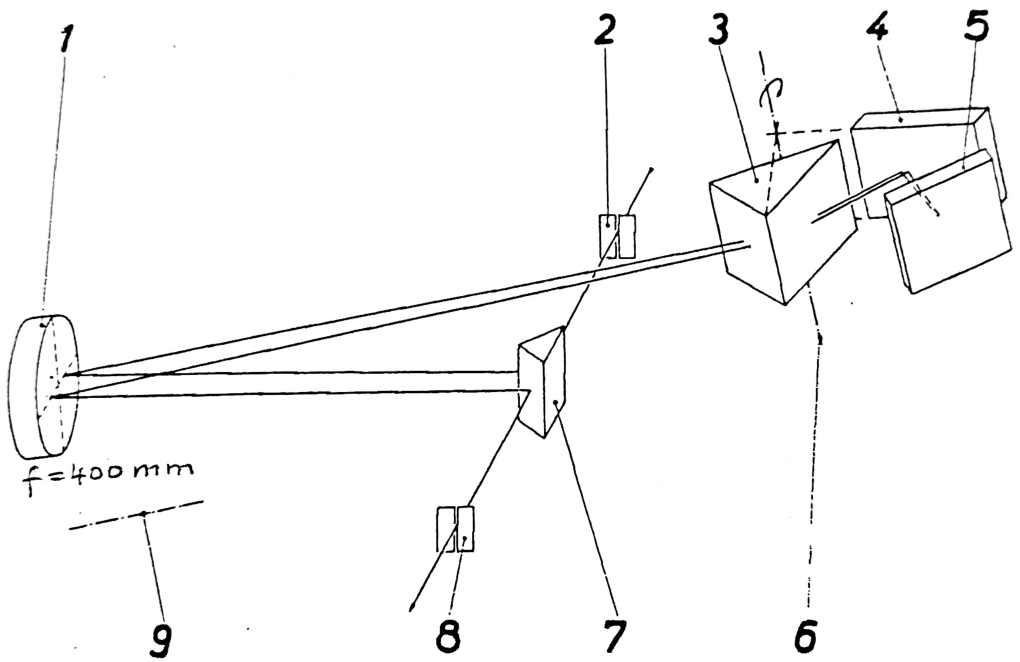
\includegraphics[width=\textwidth/2]{Bilder/SPM2.pdf}
    \caption{Spiegelkonfiguration des SPM2.}
    \label{fig:SPM2}
\end{wrapfigure}

Eintritts (2)- und Austrittsspalt (8) liegen sich gegenüber und in deren Verbindungslinie befindet sich ein Umlenkspiegel (7), der so in Verbindung mit dem Parabolspiegel (1) sowohl als Kollimator, als auch auf Kameraspiegel verwendet wird. Die Spalte befinden sich dabei jeweils in dessen Brennweite. Das Prisma (3) wird doppelt durchsetzt und ist in Verbindung mit einem Wadsworth-Spiegel (4) aufgebaut, was wie schon beim SPM1 für eine minimale Ablenkung der selektierten Wellenlänge sorgt. Entscheidend beim SPM2 ist, dass das Verändern der Prismenschraube automatisch mithilfe eines Motors geschieht, welcher durch ein angeschlossenes Labview Programm gesteuert wird. Auf dem SMP2 befindet sich eine, je nach verwendeten Prisma angepasste, Anzeige der Wellenlänge. Diese Eichung muss in die digitalisierten Daten übernommen werden. Dieses Verfahren wird in~\ref{par:EichungSPM2} beschrieben.

\begin{figure}
  \centering
  \begin{tikzpicture}[scale=0.95]

    \fill[black, rounded corners = 2mm] (6,-.3)rectangle (7.5,.3);
    \fill[black] (6.5,.3)rectangle (7,.8);
    \filldraw[draw=black, ultra thick, fill=gray] (5.3,.8)rectangle (8.2,3);

    \shadedraw[top color =black!20!white, bottom color=black!10!white, middle color=black!60!white] (-3.5,0) rectangle (4.5,0.3);
    \filldraw[thick, draw = black, fill=black!30!white] (-6.5,0) rectangle (8.5,-.3);
    \shadedraw[top color =black!20!white, bottom color=black!50!white, middle color=black!20!white] (-1,0) rectangle (1,3);
    \filldraw[rounded corners=1mm, thick, fill=gray] (-.5,1.1) rectangle (.5,2.1);
    \filldraw[rounded corners=1mm, ultra thick, fill=yellow!50!black] (-.5,1.1) -- (-.4,1.7) -- (.4,1.7) -- (.5,1.1)-- cycle;
    \filldraw[thick, fill=gray] (.6,.7) circle (.15cm);
    \filldraw[rounded corners=.5mm,thick, fill=gray] (.4,.1) rectangle (.8,.3);
    \fill[black] (.6,.2) circle (.05cm);
    \filldraw[rounded corners=.6mm,thick, fill=gray] (-.8,.1) rectangle (-.65,.4);
    \fill[rounded corners=.3mm,thick, fill=black] (-.75,.2) rectangle (-.7,.3);
    \filldraw[draw=black, thick,fill=red!70!black] (-.4,.25) circle (.07cm);
    \fill[black] (.6,.2) circle (.05cm);
    \filldraw[draw=blue, very thick, fill=black!15!white] (-6,0.025) rectangle (-4,1);
    \filldraw[draw=black, fill = gray] (-5.9,.9) rectangle (-5.3,.7);
    \filldraw[draw=black, fill = gray] (-5.9,.6) rectangle (-5.3,.4);
    \filldraw[draw=black, fill = gray] (-5.1,.8) circle (.05);
    \filldraw[draw=black, fill = gray] (-5.1,.5) circle (.05);
    \filldraw[draw=black, fill = gray] (-4.9,.9) rectangle (-4.3,.7);
    \filldraw[draw=black, fill = gray] (-4.1,.8) circle (.05);
    \filldraw[draw=black, fill = gray] (-4.1,.5) circle (.05);
    \filldraw[draw=black, fill = red] (-5.7,.25) circle (.05);
    \filldraw[draw=black, fill = blue] (-5.5,.25) circle (.05);
    \filldraw[draw=black, fill = red] (-4.7,.25) circle (.05);
    \filldraw[draw=black, fill = blue] (-4.5,.25) circle (.05);
    \filldraw[draw=black, fill = gray] (-4.9,.6) rectangle (-4.3,.4);

    \filldraw[dotted, fill=yellow!20!white](-3.3+0.08,1.2) -- +(0,0.6) -- (-1,1.5) -- cycle;
    \filldraw[dotted, fill=yellow!50!white](-3.3+0.08,1.2) -- +(0,0.6) -- (-2.3-0.1,1.5) -- cycle;
    \filldraw[draw=black, fill=gray] (-3.3,0) rectangle +(0.25,0.5);
    \filldraw[draw=black, fill=black!20!white] (-3.3+0.05,0.5) rectangle +(0.15,0.5);
    \draw[very thick] (-3.3+0.125,1) arc (190:170:3-0.125);

    \filldraw[draw=black, fill=gray] (-2.3,0) rectangle +(0.25,0.5);
    \filldraw[draw=black, fill=black!20!white] (-2.3+0.05,0.5) rectangle +(0.15,0.5);
    \filldraw[thick, fill=gray, draw=black] (-2.3-0.1,1) rectangle +(0.45,1);

    \filldraw[dotted, fill=yellow!20!white](4+0.15,1.2) -- +(0,0.6) -- (1,1.5) -- cycle;
    \filldraw[dotted, fill=yellow!50!white](4+0.15,1.2) -- +(0,0.6) -- (3.35,1.5) -- cycle;

    \filldraw[draw=black, fill=gray] (1.3,0) rectangle +(0.25,0.5);
    \filldraw[draw=black, fill=black!20!white] (1.3+0.05,0.5) rectangle +(0.15,0.9);
    \filldraw[thick, fill=gray, draw=black] (1.3-0.1,1.4) rectangle +(0.45,.2);

    \filldraw[draw=black, fill=gray] (3,0) rectangle +(0.25,0.5);
    \filldraw[draw=black, fill=black!20!white] (3+0.05,0.5) rectangle +(0.15,0.95);
    \fill[thick, fill=black] (3-0.25,1.45) rectangle +(0.6,.1);

    \filldraw[draw=black, fill=gray] (4,0) rectangle +(0.25,0.5);
    \filldraw[draw=black, fill=black!20!white] (4+0.05,0.5) rectangle +(0.15,0.5);
    \draw[very thick] (4+0.125,1) arc (-10:10:3-0.125);

    \filldraw[thick, draw = black, fill=black!30!white] (1,3.5) rectangle (8,3.8);
    \filldraw[thick, draw = black, fill=black!10!white] (1.3,3.8) rectangle (3.3,4.3);
    \filldraw[thick, draw = black, fill=black!10!white] (3.5,3.8) rectangle (6.3,5);
    \filldraw[fill=black!5!white, thick] (3.7,4.2) rectangle (4.8,4.8);
    \filldraw[fill=black!5!white, very thick] (5.8,4.5) circle (.2cm);
    \filldraw[fill=black!5!white, very thick] (5.3,4.5) circle (.2cm);
    \filldraw[thick, draw = black, fill=black!10!white] (6.5,3.8) rectangle (7.5,4.5);
    \filldraw[fill=black!5!white, very thick] (6.7,4) circle (.03cm);
    \filldraw[fill=black!5!white, very thick] (6.9,4) circle (.03cm);
    \filldraw[fill=black!5!white, very thick] (7.1,4) circle (.03cm);
    \filldraw[fill=black!5!white, very thick] (7.3,4) circle (.03cm);

    \filldraw[fill=gray, thick] (-1.5,2.4) rectangle (-1.2,2.7);
    \draw[thick] (-1.2,2.45) -- (-1,2.45);
    \draw[thick] (-1.2,2.65) -- (-1,2.65);
    \draw (-5.5,.25) to[out=-30,in=-90] (-2.3+0.05+0.075,1);
    \draw (-5.7,.25) to[out=-30,in=-90] (-2.3+0.05+0.075,1);

    \fill (-1.2,2.3) -- +(0.1,0) -- (-1.15,1.75) -- cycle;
    \fill (-1.2,1.3) -- +(0.1,0) -- (-1.15,1.85) -- cycle;
    \draw (-1.15, 1.8) -- (-1,1.8);
    \draw (1,3.65) to[out=200,in=150] (3-0.25,1.5);
    \draw (3.3,4.05) to[out=0,in=180] (3.5,4.4);
    \draw (3.3,4.05) to[out=0,in=180] (3.5,4.4);
    \draw (6.3,4.4) to[out=0,in=180] (6.7,4);
    \draw (7.5,4.4) to[out=0,in=90] (7.7,3);

    \node (A) at (1.4,-.7){\footnotesize Probe};
    \node (A) at (3.15,-.7){\footnotesize Detektor};
    \node (A) at (6.75,-.7){\footnotesize Rechner};
    \node (A) at (-2.2,-.7){\footnotesize Wolframlampe};
    \node (A) at (-5,1.4){\footnotesize Spannungsquelle};
    \node (A) at (-3.1,2.3){\footnotesize Hohlspiegel};
    \node (A) at (-1.4,3.2){\footnotesize Motor};
    \node (A) at (7.3,4.7){\footnotesize AD-Wandler};
    \node (A) at (4.9,5.2){\footnotesize Lock-In-Verstärker};
    \node (A) at (2.3,4.5){\footnotesize Vorverstärker};
  \end{tikzpicture}
  \caption{Schematischer Aufbau des SPM2 Prismenspektrographen.}
\end{figure}


\subsection{Lock-In-Verstärker}
Lock-in-Verstärker sind wesentliche Bestandteile zahlreicher hochempfindlicher Messaufbauten, denn sie bieten die Möglichkeit, Signale schwacher Amplitude aus dem Rauschen gewinnen zu können und zu messen.
Dazu wird die Strahlung periodisch unterbrochen bzw. moduliert. So gelingt es, das Signal gut von der Umgebungsstrahlung unterscheiden zu können, sowie es leichter elektronisch verarbeiten zu können. Ein Lock-In-Verstärker ist folgendermaßen aufgebaut: zuerst befindet sich ein Modulator mit Lichtschranke im Strahlengang. Dahinter folgt ein Empfänger (z.B. wie im Versuch ein Vakuumthermoelement). Von dort aus gelangt das Signal in einen aus drei Komponenten aufgebauten Selektivverstärker, bestehend aus einem Breitbandverstärker, einem TT-Filter in Gegenkopplung und einem Nachverstärker. Anschließend passiert das Signal einen Verstärker mit Relais, der als phasenempfindlicher Gleichrichter wirkt, sowie ein RC-Glied, durch welches das Signal geglättet wird. Der Verlauf des Signals ist in Abbildung \ref{fig:Lock-Inn} dargestellt.

\begin{figure}[ht]
    \centering
    \newcommand\PhasenverschiebungLinks{0} % In Grad [°]
	\pgfplotsset{height=0.3\textheight}
	\begin{tikzpicture}[baseline]
	\begin{axis}[
	title={$\Delta \varphi = \SI{\PhasenverschiebungLinks}{\degree}$},
	x=1cm,
	y=0.5cm,
	clip=false,
	xlabel={$t$},
	ylabel={$U$},
	%xtick=\empty,
	%ytick=\empty,
	xmin=-0.2,
	xmax=2.2,
	ymin=-8.8	,
	ymax=1.3,
	xtick=\empty,
	ytick=\empty,
	axis x line=middle,
	axis y line=middle,
	scaled ticks=false,
	every axis x label/.style={
		at={(ticklabel* cs:1)},
		anchor=west,
	},
	every axis y label/.style={
		at={(ticklabel* cs:1)},
		anchor=east,
	},
	footnotesize,
	]
	\addplot [thick,red,mark=none,domain=0:2,samples=200] { sin(deg(2*pi*x)) }; % Signal
	\addplot [thick,blue,mark=none,domain=0:2,samples=200] { (sign(sin(deg(2*pi*x) + \PhasenverschiebungLinks)))/2 + 0.5 }; % Referenz mit Phasenverschiebung
	\draw [-stealth] (-0.2,-2.5) -- (2.2,-2.5);
	\addplot [thick,violet,mark=none,domain=0:2,samples=200] { sin(deg(2*pi*x))*((sign(sin(deg(2*pi*x) + \PhasenverschiebungLinks)))/2 + 0.5) - 2.5 }; % Phasenempfindliche Einweg-Gleichrichtung
	\draw [-stealth] (-0.2,-5) -- (2.2,-5);
	\addplot [thick,violet,mark=none,domain=0:2,samples=200] { sin(deg(2*pi*x))*((sign(sin(deg(2*pi*x) + \PhasenverschiebungLinks)))/2 + 0.5) + sin(deg(2*pi*x) + 180)*((sign(sin(deg(2*pi*x) + \PhasenverschiebungLinks + 180)))/2 + 0.5) - 5 }; % Phasenempfindliche Einweg-Gleichrichtung gleichgerichtet
	\draw [-stealth] (-0.2,-7.5) -- (2.2,-7.5);
	\addplot [ultra thick,violet,mark=none] coordinates { (0,{-7.5+cos(\PhasenverschiebungLinks)/sqrt(2)}) (2,{-7.5+cos(\PhasenverschiebungLinks)/sqrt(2)}) };
	\node [left] at (-0.2,+0.4) {\textcolor{blue}{Referenz}};
	\node [left] at (-0.2,-0.4) {\textcolor{red}{Signal}};
	\node [left] at (-0.2,-2.1) {Einweg-};
	\node [left] at (-0.2,-2.9) {gleichrichtung};
	\node [left] at (-0.2,-4.6) {Zweiweg-};
	\node [left] at (-0.2,-5.4) {gleichrichtung};
	\node [left] at (-0.2,-7.1) {nach};
	\node [left] at (-0.2,-7.9) {Glättung};
	\end{axis}
	\end{tikzpicture}
	% MITTE
	\newcommand\PhasenverschiebungMitte{90} % In Grad [°]
	\begin{tikzpicture}[baseline]
	\begin{axis}[
	title={$\Delta \varphi = \SI{\PhasenverschiebungMitte}{\degree}$},
	x=1cm,
	y=0.5cm,
	xlabel={$t$},
	ylabel={$U$},
	%xtick=\empty,
	%ytick=\empty,
	xmin=-0.2,
	xmax=2.2,
	ymin=-8.8	,
	ymax=1.3,
	xtick=\empty,
	ytick=\empty,
	axis x line=middle,
	axis y line=middle,
	scaled ticks=false,
	every axis x label/.style={
		at={(ticklabel* cs:1)},
		anchor=west,
	},
	every axis y label/.style={
		at={(ticklabel* cs:1)},
		anchor=east,
	},
	footnotesize,
	]
	\addplot [thick,red,mark=none,domain=0:2,samples=200] { sin(deg(2*pi*x)) }; % Signal
	\addplot [thick,blue,mark=none,domain=0:2,samples=200] { (sign(sin(deg(2*pi*x) + \PhasenverschiebungMitte)))/2 + 0.5 }; % Referenz mit Phasenverschiebung
	\draw [-stealth] (-0.2,-2.5) -- (2.2,-2.5);
	\addplot [thick,violet,mark=none,domain=0:2,samples=200] { sin(deg(2*pi*x))*((sign(sin(deg(2*pi*x) + \PhasenverschiebungMitte)))/2 + 0.5) - 2.5 }; % Phasenempfindliche Einweg-Gleichrichtung
	\draw [-stealth] (-0.2,-5) -- (2.2,-5);
	\addplot [thick,violet,mark=none,domain=0:2,samples=200] { sin(deg(2*pi*x))*((sign(sin(deg(2*pi*x) + \PhasenverschiebungMitte)))/2 + 0.5) + sin(deg(2*pi*x) + 180)*((sign(sin(deg(2*pi*x) + \PhasenverschiebungMitte + 180)))/2 + 0.5) - 5 }; % Phasenempfindliche Einweg-Gleichrichtung gleichgerichtet
	\draw [-stealth] (-0.2,-7.5) -- (2.2,-7.5);
	\addplot [ultra thick,violet,mark=none] coordinates { (0,{-7.5+cos(\PhasenverschiebungMitte)/sqrt(2)}) (2,{-7.5+cos(\PhasenverschiebungMitte)/sqrt(2)}) };
	\end{axis}
	\end{tikzpicture}
	% RECHTS
	\newcommand\PhasenverschiebungRechts{180} % In Grad [°]
	\begin{tikzpicture}[baseline]
	\begin{axis}[
	title={$\Delta \varphi = \SI{\PhasenverschiebungRechts}{\degree}$},
	x=1cm,
	y=0.5cm,
	xlabel={$t$},
	ylabel={$U$},
	%xtick=\empty,
	%ytick=\empty,
	xmin=-0.2,
	xmax=2.2,
	ymin=-8.8	,
	ymax=1.3,
	xtick=\empty,
	ytick=\empty,
	axis x line=middle,
	axis y line=middle,
	scaled ticks=false,
	every axis x label/.style={
		at={(ticklabel* cs:1)},
		anchor=west,
	},
	every axis y label/.style={
		at={(ticklabel* cs:1)},
		anchor=east,
	},
	footnotesize,
	]
	\addplot [thick,red,mark=none,domain=0:2,samples=200] { sin(deg(2*pi*x)) }; % Signal
	\addplot [thick,blue,mark=none,domain=0:2,samples=200] { (sign(sin(deg(2*pi*x) + \PhasenverschiebungRechts)))/2 + 0.5 }; % Referenz mit Phasenverschiebung
	\draw [-stealth] (-0.2,-2.5) -- (2.2,-2.5);
	\addplot [thick,violet,mark=none,domain=0:2,samples=200] { sin(deg(2*pi*x))*((sign(sin(deg(2*pi*x) + \PhasenverschiebungRechts)))/2 + 0.5) - 2.5 }; % Phasenempfindliche Einweg-Gleichrichtung
	\draw [-stealth] (-0.2,-5) -- (2.2,-5);
	\addplot [thick,violet,mark=none,domain=0:2,samples=200] { sin(deg(2*pi*x))*((sign(sin(deg(2*pi*x) + \PhasenverschiebungRechts)))/2 + 0.5) + sin(deg(2*pi*x) + 180)*((sign(sin(deg(2*pi*x) + \PhasenverschiebungRechts + 180)))/2 + 0.5) - 5 }; % Phasenempfindliche Einweg-Gleichrichtung gleichgerichtet
	\draw [-stealth] (-0.2,-7.5) -- (2.2,-7.5);
	\addplot [ultra thick,violet,mark=none] coordinates { (0,{-7.5+cos(\PhasenverschiebungRechts)/sqrt(2)}) (2,{-7.5+cos(\PhasenverschiebungRechts)/sqrt(2)}) };
	\end{axis}
\end{tikzpicture}

    \caption{Phasenabhängigkeit der Gleichrichtung im Zeitverlauf.}
    \label{fig:Lock-Inn}
\end{figure}

So gelingt es, Signale, deren Phasenlage gegenüber dem Referenzsignal nicht konstant bzw. deren Frequenz nicht mit dem Referenzsignal übereinstimmt herauszufiltern, da diese sich nach der Glättung zu Null ergeben.

\subsection{Auflösung und spektralen Spaltbreite}\label{sec:spektraleSpaltbreite}
\subsubsection{Auflösung}
Um die Auflösung der Abbildung mit einem Prismenspektrometer herzuleiten, werden geometrische Überlegungen angestellt. Grundlage der Herleitung ist die Tatsache, dass das Strahlenbündel beim Passieren des Prismas eingeschränkt wird, weshalb dieses als Spalt wirkt und es deshalb zu Beugungsphänomenen kommt. Resultat dieser Herleitung ist das theoretische beugungsbegrenzte Auflösungsvermögen eines Prismas
\begin{align}
  R = - P \dv{n}{\lambda}
\end{align}
wobei $P$ die Basislänge des Prismas ist. \\
Das reale Auflösungsvermögen ergibt sich dann zu
\begin{align}
  \frac{\Delta\lambda}{\lambda}=\frac{\lambda R}{\lambda+\Phi b}
\end{align}
mit $\Phi =$ Kollimatorspiegeldurchmesser/Brennweite und $b=$ Spaltbreite.

\subsubsection{Spektrale Spaltbreite}
Bei Messungen dieser Art liegt immer eine konstante geometrische Spaltbreite vor. Aufgrund der Winkeldispersion passieren diesen Spalt nicht nur Strahlen einer Wellenlänge, sondern immer die eines ganzen Wellenlängenintervalls. Dabei zeigt die Abhängigkeit der spektralen Strahlungsleistung eines engen Wellenlängenintervalls nach dem Durchgang durch einen Spalt einen charakteristischen Verlauf. Bei gleicher Eintritts- und Austrittsspaltbreite kann diese durch eine Dreiecksfunktion mit Maximum bei der eingestellten Wellenlänge beschrieben werden. Diese Funktion gibt eine Wahrscheinlichtkeitsaussage über denjenigen Strahlungsanteil, der den Detektor erreicht, an. \\
Das Wellenlängenintervall, das diese immer gleiche geometrische Spaltbreite passiert ist jedoch auf Grund der Winkeldispersion des Prismas nicht immer gleich groß, sondern abhängig von dem Wellenlängenbereich, der betrachtet wird. So ist bei der Aufnahme der Spektralverteilung zu beachten, dass die Strahlungsdichte aus dem Planck-Gesetz von einem konstanten Wellenlängenintervall ausgeht. Um die Messwerte als mit den Theoriewerten in Deckung zu bringen, ist eine Korrektur durch Division $\Delta \lambda$ = const$\cdot \dv{\lambda}{l}$ nötig, wobei $\dd{l}$ die infinitesimale Änderung der Schraubeneinstellung darstellt.

\subsection{Empfänger}\label{sec:Empfänger)}
\subsubsection{Thermische Detektoren}
Thermische Detektoren beruhen auf der Messung von Effekten, die aufgrund der Temperaturänderung nach Strahlungseinfall enstehen. Deshalb ist das so entstehende Photosignal nur vom auftreffenden Strahlungsfluss abhängig und deshalb wellenlängenunabhängig. \\
Je nach ausgenutzten Effekt unterscheidet man unterschiedliche thermische Detektoren. Das \emph{Thermoelement} nutzt die temperaturabhängige Änderung der Thermospannung, die sich an der Kontaktstelle zweier verschiedener Materialien ergibt, da deren Ferminiveaus sich bei Änderung der Temperatur materialspezifisch verschieben.
Die Widerstandsänderung eines elektrischen Leiters aufgrund der Temperaturänderung durch Strahlungsabsorption zu messen, ist das Prinzip des \emph{Bolometers}.
\emph{Pyroelektrische Strahlunsgempfänger} nutzen den Effekt aus, dass bei ferromagnetischen Materialien unterhalb des \textsc{Curie}-Punktes Polarisationsänderungen auftreten. Die bei bestimmten Materialien auftretende spontane Polarisation kann als elektrisches Signal gemessen werden. Der \emph{Golay-Detektor} beruht auf der Änderung des Gasdruckes durch die Absorptionswärme. Diese verformt einen flexiblen Spiegel, der Teil eines optisches Systems ist, welches in Folge dessen eine Änderung registriert.

\subsubsection{Photodetektoren}
Auch hier können zwei unterschiedliche Effekte genutzt werden.\\
\emph{Photoleitfähigkeit}: Die einfallende Strahlung erzeugt Elektronen-Loch-Paare. Dadurch ändert sich die elektrische Leitfähigkeit eines Halbleiters beim Einfall von Strahlung. Das Photosignal wird dann entweder als Spannungsänderung über einen Widerstand abgenommen oder als Stromänderung gemessen. \\
\emph{Photospannung}: Detektoren, die auf diesem Effekt beruhen, bestehen aus einer n- sowie einer p-Schicht. Durch die einfallende Strahlung bildet sich ein Ladungsträgerpaar, welches über die n- und p-Grenzschicht getrennt wird und damit eine elektrische Spannung entsteht, die gemessen wird. \\
Photodetektoren haben eine höhere Empfindlichkeit, als thermische Detektoren, sind aber aufgrund der Notwenigkeit der Überwindung der Bandlücke wellenlängenabhängig in ihrer Empfindlichkeit.

\subsubsection{Spektrale Empfindlichkeit}
Weil thermische Empfänger ausschließlich auf Effekten beruhen, die aufgrund einer Temperaturänderung auftreten, ist die Empfindlichkeit dieser Empfänger wellenlängenunabhängig. Anders verhält es sich mit den Halbleiterdetektoren. Da es bei diesen nur dann zur Entstehung eines Signals kommen kann, wenn die Energie aufgebracht wird, um ein Elektron vom Valenz- ins Leitungsband zu heben, also wenn mindestens die Bandlückenenergie aufgebracht wird, zeigen diese Detektoren eine Wellenlängenabhängigkeit. \\
Die spektrale Empfindlichkeit $r(\lambda)$ eines Empfängern bei der Wellenlänge $\lambda$ ist definiert als Verhältnis der vom Empfänger abgegebenen Messgröße $M(\lambda)$ (z.B. Spannung, Strom, Ausschlag) zu der Strahlungsleistung $P_S(\lambda)$:
\begin{align}
  r(\lambda) = \frac{M(\lambda)}{P_S(\lambda)}
\end{align}
Da die Empfindlichkeit des Thermoelements, wie in Abschnitt \ref{sec:Empfänger} verdeutlicht, wellenlängenunabhängig ist, gibt der Verlauf der Messung mit dem Thermoelement den Verlauf von $P_S(\lambda)$ wieder. So ergibt sich, dass die $r(\lambda)$ gemessen werden kann, indem die Messung einmal mit dem zu vermessenden (Halbleiter-)Empfänger, sowie anschließend mit dem Thermoelement durchgeführt wird und die spektrale Empfindlichkeit dann berechnet werden kann als
\begin{align}
  r(\lambda) = \frac{A_\text{Empfänger}(\lambda)}{A_\text{Thermoelement}(\lambda)}
\end{align}

wobei A der Ausschlag des Galvanometers ist.

\subsection{Wechselwirkungen im Infrarotbereich}\label{sec:Wechselwirkungen}

Damit Molekülübergänge im infraroten Bereich stattfinden können, müssen die beteiligten Moleküle ein permanentes oder induziertes Dipolmoment aufweisen. Moleküle, die diese Eigenschaft erfüllen, werden \emph{infrarotaktiv} bezeichnet. Für homonukleare, symmetrische Moleküle wie \ce{N2}, \ce{O2} verschwindet das Kerndipolmoment und es können keine Schwingungsbanden im IR angeregt werden. Aus diesem Grund tragen diese Gase nicht zum Treibhauseffekt der Erde bei, im Gegensatz zu \ce{H2O} oder \ce{CO2}, welche die von der Erde emittierte IR-Strahlung absorbieren und reemittieren.

Damit ein Photon von einem Molekül absorbiert werden kann, muss ein entsprechender Schwingungsübergang nach der Quantenmechanik erlaubt sein. Für Schwingungs- Rotationsübergänge gelten daher gewisse Auswahlregeln ($\Delta J = \pm 1, \Delta m = 0, \pm 1$). Eine beispielhafte Darstellung eines solchen Spektrums zeigt Abbildung~\ref{Rotationsschwingung}. Die Wellenlängenunterschiede von Rotationsschwingungen sind meist jedoch zu klein, damit diese von einem Prismenspektrometer aufgelöst werden können.

\begin{figure}[htp]
  \centering
  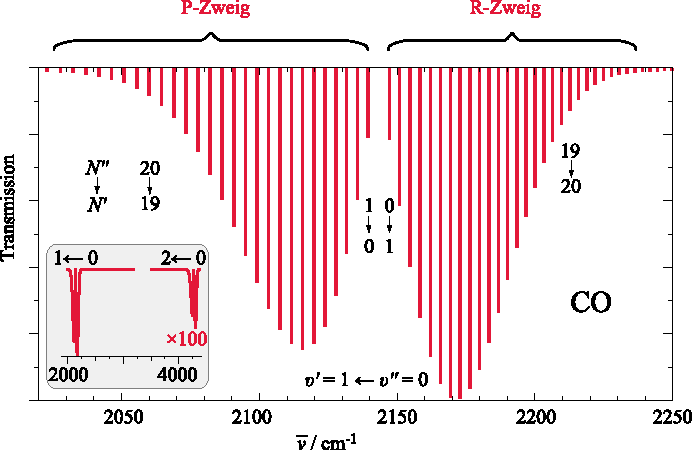
\includegraphics{Bilder/Rotationsschwingung.pdf}
  \caption{Simulierte Rotationsschwingungsbande für \ce{CO} im elektronischen Grundzustand nach~\cite{Hertel}. Es findet ein Schwingungsübergang bei einer Temperatur von \SI{293}{\kelvin} statt. Der Einschub zeigt auch die zweite harmonische ($\nu=2 \to \nu=0$).}
\end{figure}

Für komplexere Moleküle werden die Schwingungsübergänge zu verschiedenen Gruppen zusammengefasst. So können einerseits Valenzschwingungen entlang der Bindungsachse auftreten (Streckschwingungen) oder Schwingungen mit Deformation der Kernverbindungsachse (Deformationsschwingungen).

In Halbleitermaterialien sind insbesondere Interbandübergänge möglich, die auf dem inneren photoelektrischen Effekt beruhen. Hier werden die Elektronen aus dem Valenzband in das Leitungsband angehoben. Die Voraussetzung dafür ist, dass die Energie des absorbierten Photons größer ist, als die Bandlückenenergie. Weiterhin ist es möglich, dass in Materialien, die im sichtbaren transparent sind, im IR-Bereich Gitterschwingungen auftreten, die beispielsweise die Transparenz von Glas reduzieren.

Im Versuch werden zur Untersuchung verschiedener Proben Transmissionsspektren aufgenommen. Die Transmission eines homogenen Stoffes mit geringem Reflexionsvermögen wird beschrieben durch das \textsc{Lambert-Beer}'sche Gesetz:
\begin{align}
  T=\frac{I_D}{I_0}=(1-R)^2\cdot\exp(-Kd)
\end{align}
wobei $K$ die Extinktionskonstante ist und $d$ die Schichtdicke angibt. Die Größe $R$ beschreibt das Reflexionsvermögen.

Zur Auswertung von Spektren in Reflexionsmessung wird das Reflexionsvermögen heragezogen. Bei quasi senkrechtem Lichteinfall berechnet sich das Reflexionsvermögen nach den \textsc{Fresnel}'schen Formeln an einer Grenzfläche bei Anwesenheit von Absorption zu

\begin{align}
  R(\lambda)=\frac{N_1(\lambda)-N_2(\lambda)}{N_1(\lambda)+N_2(\lambda)}
\end{align}

mit dem komplexen Brechungsindex $N(\lambda) = n(\lambda)+\mathrm{i}k(\lambda)$  und dem Absorptionsindex $k$.
Werden als Medien Luft (N=1) und ein beliebiges Medium mit $N_2 = N$ verwendet, ergibt sich für das Reflexionsvermögen
\begin{align}
  R(\lambda)=\frac{(n-1)^2+k^2}{(n+1)^2+k^2}
\end{align}

Daraus wird ersichtlich, dass in den Wellenlängenbereichen, wo Absorption auftritt, also $n$ und $k$ groß sind, auch das Reflexionsvermögen groß wird.

% *********************************************
% ***** KAPITEL 4 *****************************
% *********************************************
\newpage
\section{Ergebnisse und Diskussion}\label{sec:ErgebnisseUndDiskussion}
% \begin{figure}[htp]
  \centering
  \begin{tikzpicture}
    \begin{axis}[disabledatascaling, width=\textwidth, height=6cm, ylabel=Wellenlänge in \si{\nano\metre}, xlabel=Winkel  $\varphi$ in rad, xmin = 0, xmax=999, xtick={}]
      \addplot[color=red,mark=x] coordinates {
		(0,500)
    (90,600)
		(143,700)
		(184,800)
    (219,900)
    (247,1000)
    (273,1100)
    (296,1200)
    (320,1300)
    (343,1400)
    (367,1500)
    (391,1600)
    (416,1700)
    (444,1800)
    (472,1900)
    (500,2000)
    (532,2100)
    (564,2200)
    (598,2300)
    (634,2400)
    (669,2500)
    (708,2600)
    (748,2700)
    (790,2800)
    (833,2900)
    (881,3000)
    (929,3100)
    (979,3200)
	};
    \end{axis}
  \end{tikzpicture}
\end{figure}

\subsection{Aufbau und Wellenlängeneichung eines Prismenmonochromators (SPM1)}
\subsubsection{Justage des Prismenmonochromators in Wadsworth-Anordung}
Um den Prismenmonochromator in Wadsworth-Anordnung zu justieren wird eine Quecksilberdampflampe verwendet. Diese wird so justiert, dass der Fokuspunkt ihres Strahls auf dem Eintrittsspalt lokalisiert ist. Gleichzeitig ist darauf zu achten, dass der erste Spiegel möglichst voll ausgeleuchtet ist. Auch der zweite Spiegel wird so justiert, dass die aus dem Prisma kommenden Strahlen auf diesen fallen. Die Austrittsblende agiert als Monochromator. Mit der Kombination aus Thermoelement und Galvanometer kann auch bei optimaler Justage kein Ausschlag gemessen werden, weshalb eine Photodiode als Empfänger genutzt wird. Diese wird so positioniert, dass der Detektor sich im Fokuspunkt des Strahls befindet.

\subsubsection{Eichung und Auflösungsvermögen}
Die Skale der Prismenverstellung wird bezüglich der Wellenlänge mit Hilfe der Linien der Quecksilberdampflampe geeicht. Zum Eichen wird bei der grünen Spektrallinie begonnen, da die Photodiode bei dieser eine bessere Empfindlichkeit aufweist, als für den blauen Spektralbereich. Dazu wird das Prisma so eingestellt, dass die grüne Spektrallinie den Austrittsspalt passieren kann. Aufgrund der bekannten Daten für die Spektrallinien der Quecksilberdampflampe kann dem in dem Bereich gefunden Maxima und dem dazugehörigem am Rad der Prismeneinstellung abgelesenen Skalenwert eine Wellenlänge zugeordnet werden. Die unterschiedlichen Einstellungen des Prismas werden durchgefahren und jeweils bei den gefundenen Maxima kann dem zugehörigen Skalenwert nach gleichem Prinzip wie oben beschrieben eine Wellenlänge zugeordnet werden. Die erhaltenen Datenpaare können dargestellt und gefittet werden, woraus eine Funktion erhalten wird, die den am Rad der Prismeneinstellung abgelesenen Skalenwerten eine Wellenlänge zuordnet.
\begin{figure}[htp]
    \centering
        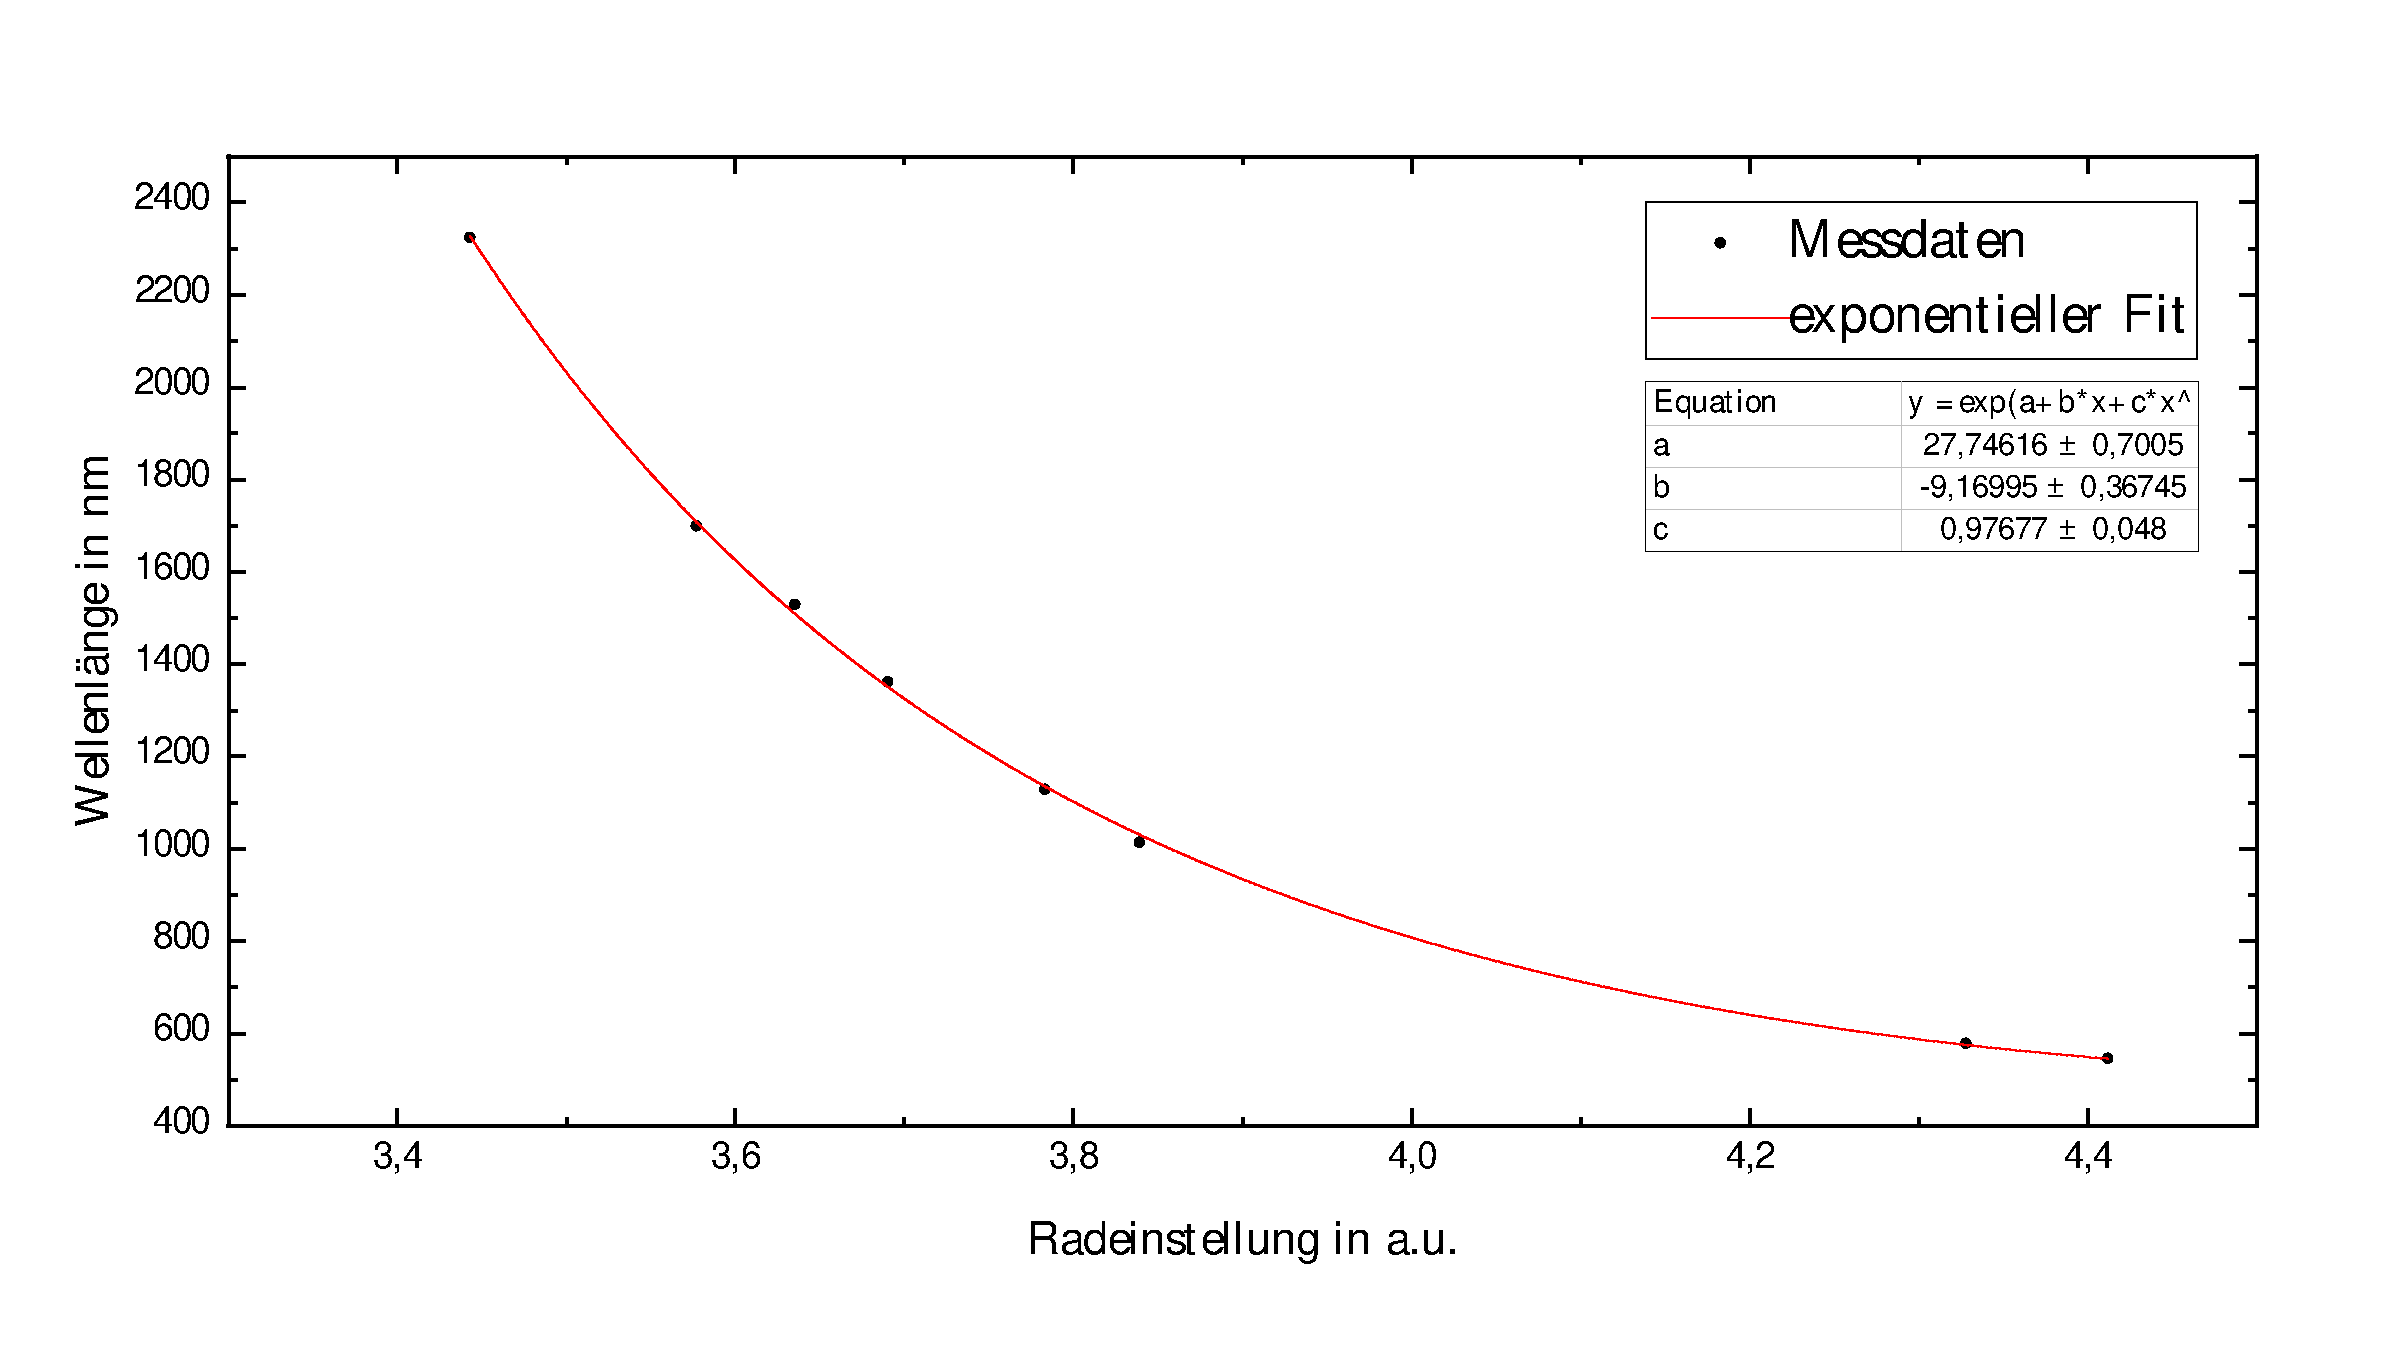
\includegraphics[width=0.9\textwidth]{Bilder/Eichung_SPM1_mitQuecksilberdapflampe.pdf}
    \caption{Eichung der Prismenverstellung}
    \label{fig:EichungSPM1}
\end{figure}

Zur Abschätzung der Auflösung wird die Natriumdampflampe verwendet. Der Aufbau wird auf die Doppellinie des Natriums eingestellt. Anstelle des Spiegels zwei wird ein Fernrohr aufgebaut, um die Linien direkt beobachten zu können. Trotz kleinster Öffnungsweite der Blenden können die zwei gelben Linien des Natriums, welche sich bei \SI{588.9951}{\nano\meter} und bei \SI{589.5924}{\nano\meter} befinden, nicht unterschieden werden.

\subsection{Messungen anhand des Wolframlampenspektrums}
\subsubsection{Spektrale Empfindlichkeit eines Halbleiterempfängers}
Die spektrale Empfindlichkeit eines Empfängers kann nach Abschnitt \ref{sec:Empfänger)} berechnet werden, indem das Signal mit dem Empfänger, sowie mit einem Thermoelement vermessen  und das Verhältnis der Messwerte gebildet wird. Dazu wird nach der Austrittsblende einmal das Thermoelement, sowie bei anschließenden Messungen ein InGaAs-Halbleiterdetektor und ein Si-Halbleiterdetektor in den Fokuspunkt des austretenden Strahl positioniert. Das Signal der Halbleiterdetektoren wird mit einem Verstärker verstärkt und anschließend am Multimeter abgelesen, während das Signal des Thermoelements mit dem Galvanometer vermessen wird. Bei Letzterem ist das Ablesen nur mit einer sehr schlechten Auflösung möglich, weshalb vorallem kleine Signale schlecht vermessen bzw. überhaupt detektiert werden können. So ergibt sich, dass nur die Bereich der Empfindlichkeitskurven vermessen werden können, in denen das Signal des Thermoelements sich von Null unterscheiden lässt, weshalb die erhaltenen Empfindlichkeitskurven nur unvollständig vermessen werden konnten. Eine vollständige Vermessung kann mit einem Messgerät mit besserer Auflösung vorallem in niedrigen Signalbereichen realisiert werden.

\begin{figure}[htp]
  \centering
  \begin{subfigure}{0.9\textwidth}
    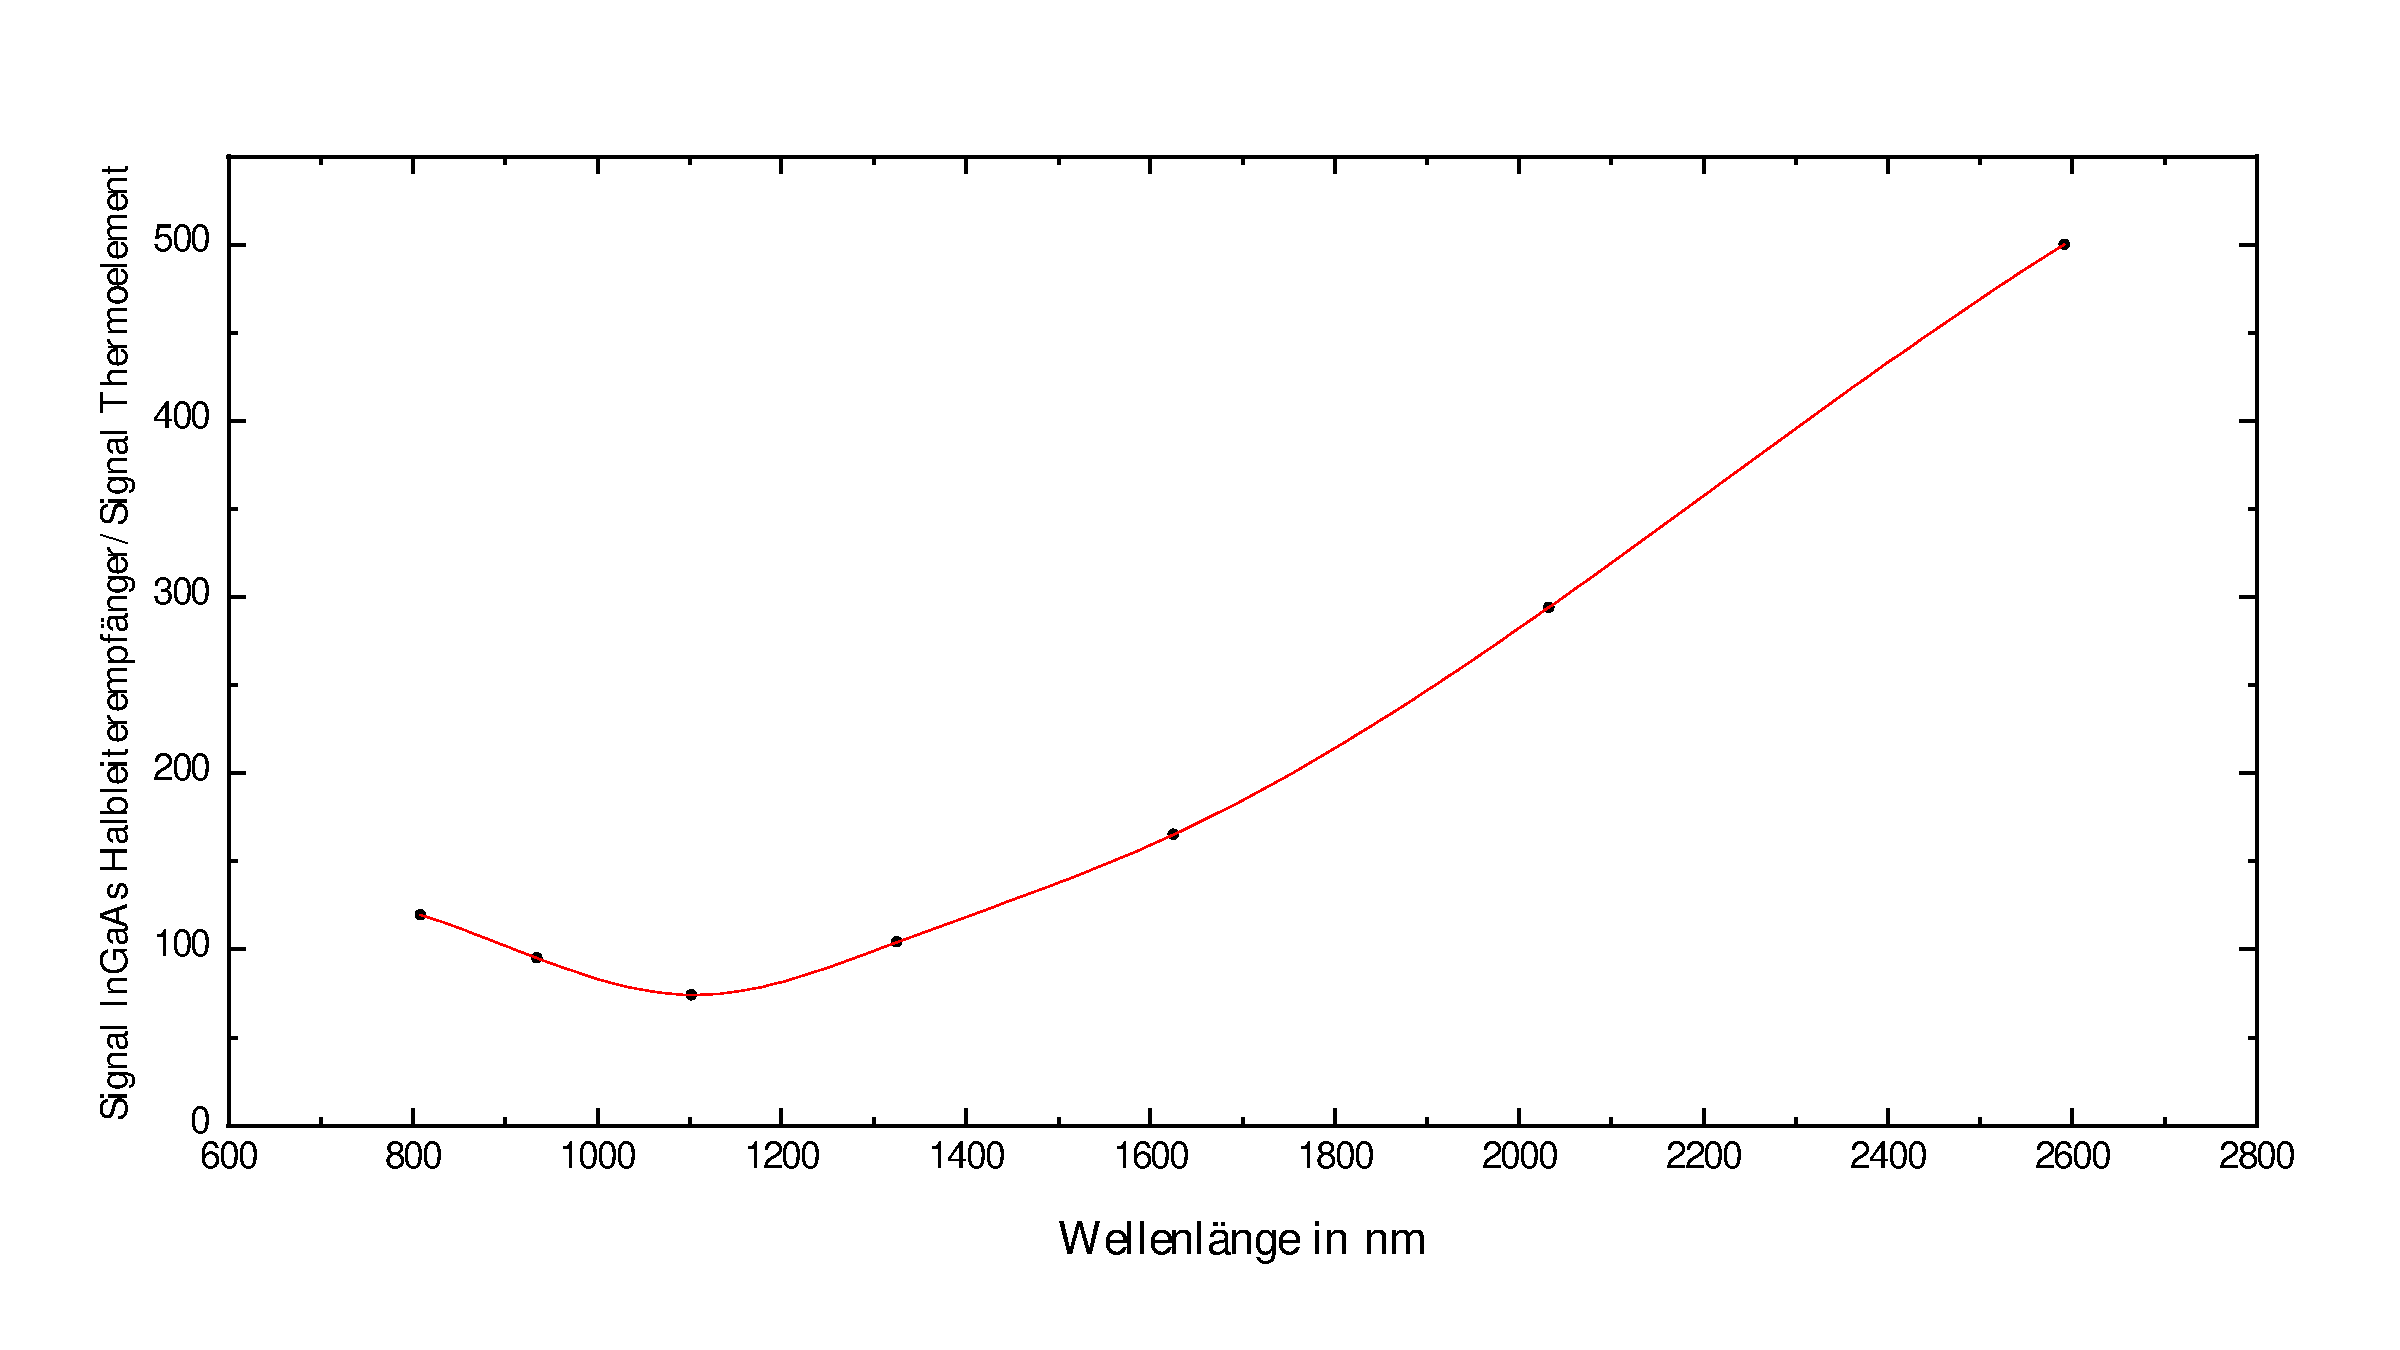
\includegraphics[width=\textwidth]{Bilder/Empfindlichkeit_InGaAs.pdf}
    \caption{aus Messdaten}
  \end{subfigure}
  \begin{subfigure}{0.7\textwidth}
    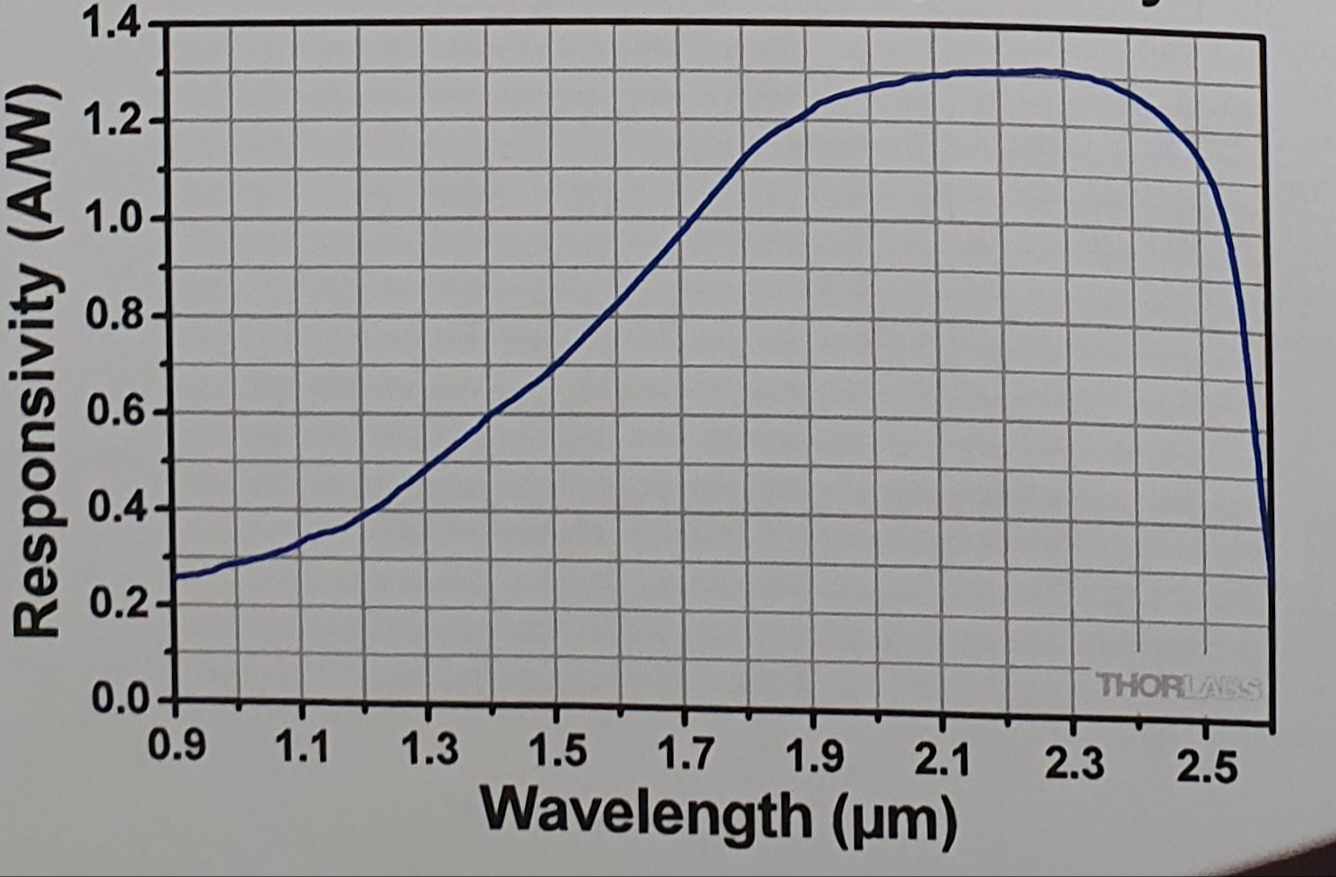
\includegraphics[width=\textwidth]{Bilder/Empfindlichkeit_InGaAsHalbleiter_manual.jpeg}
    \caption{vom Hersteller}
  \end{subfigure}\hspace{1cm}
  \caption{spektrale Empfindlichkeit eines InGaAs-Halbleiterdetektors}
  \label{fig:Empf_InGaAs}
\end{figure}

\begin{figure}[htp]
  \centering
  \begin{subfigure}{0.9\textwidth}
    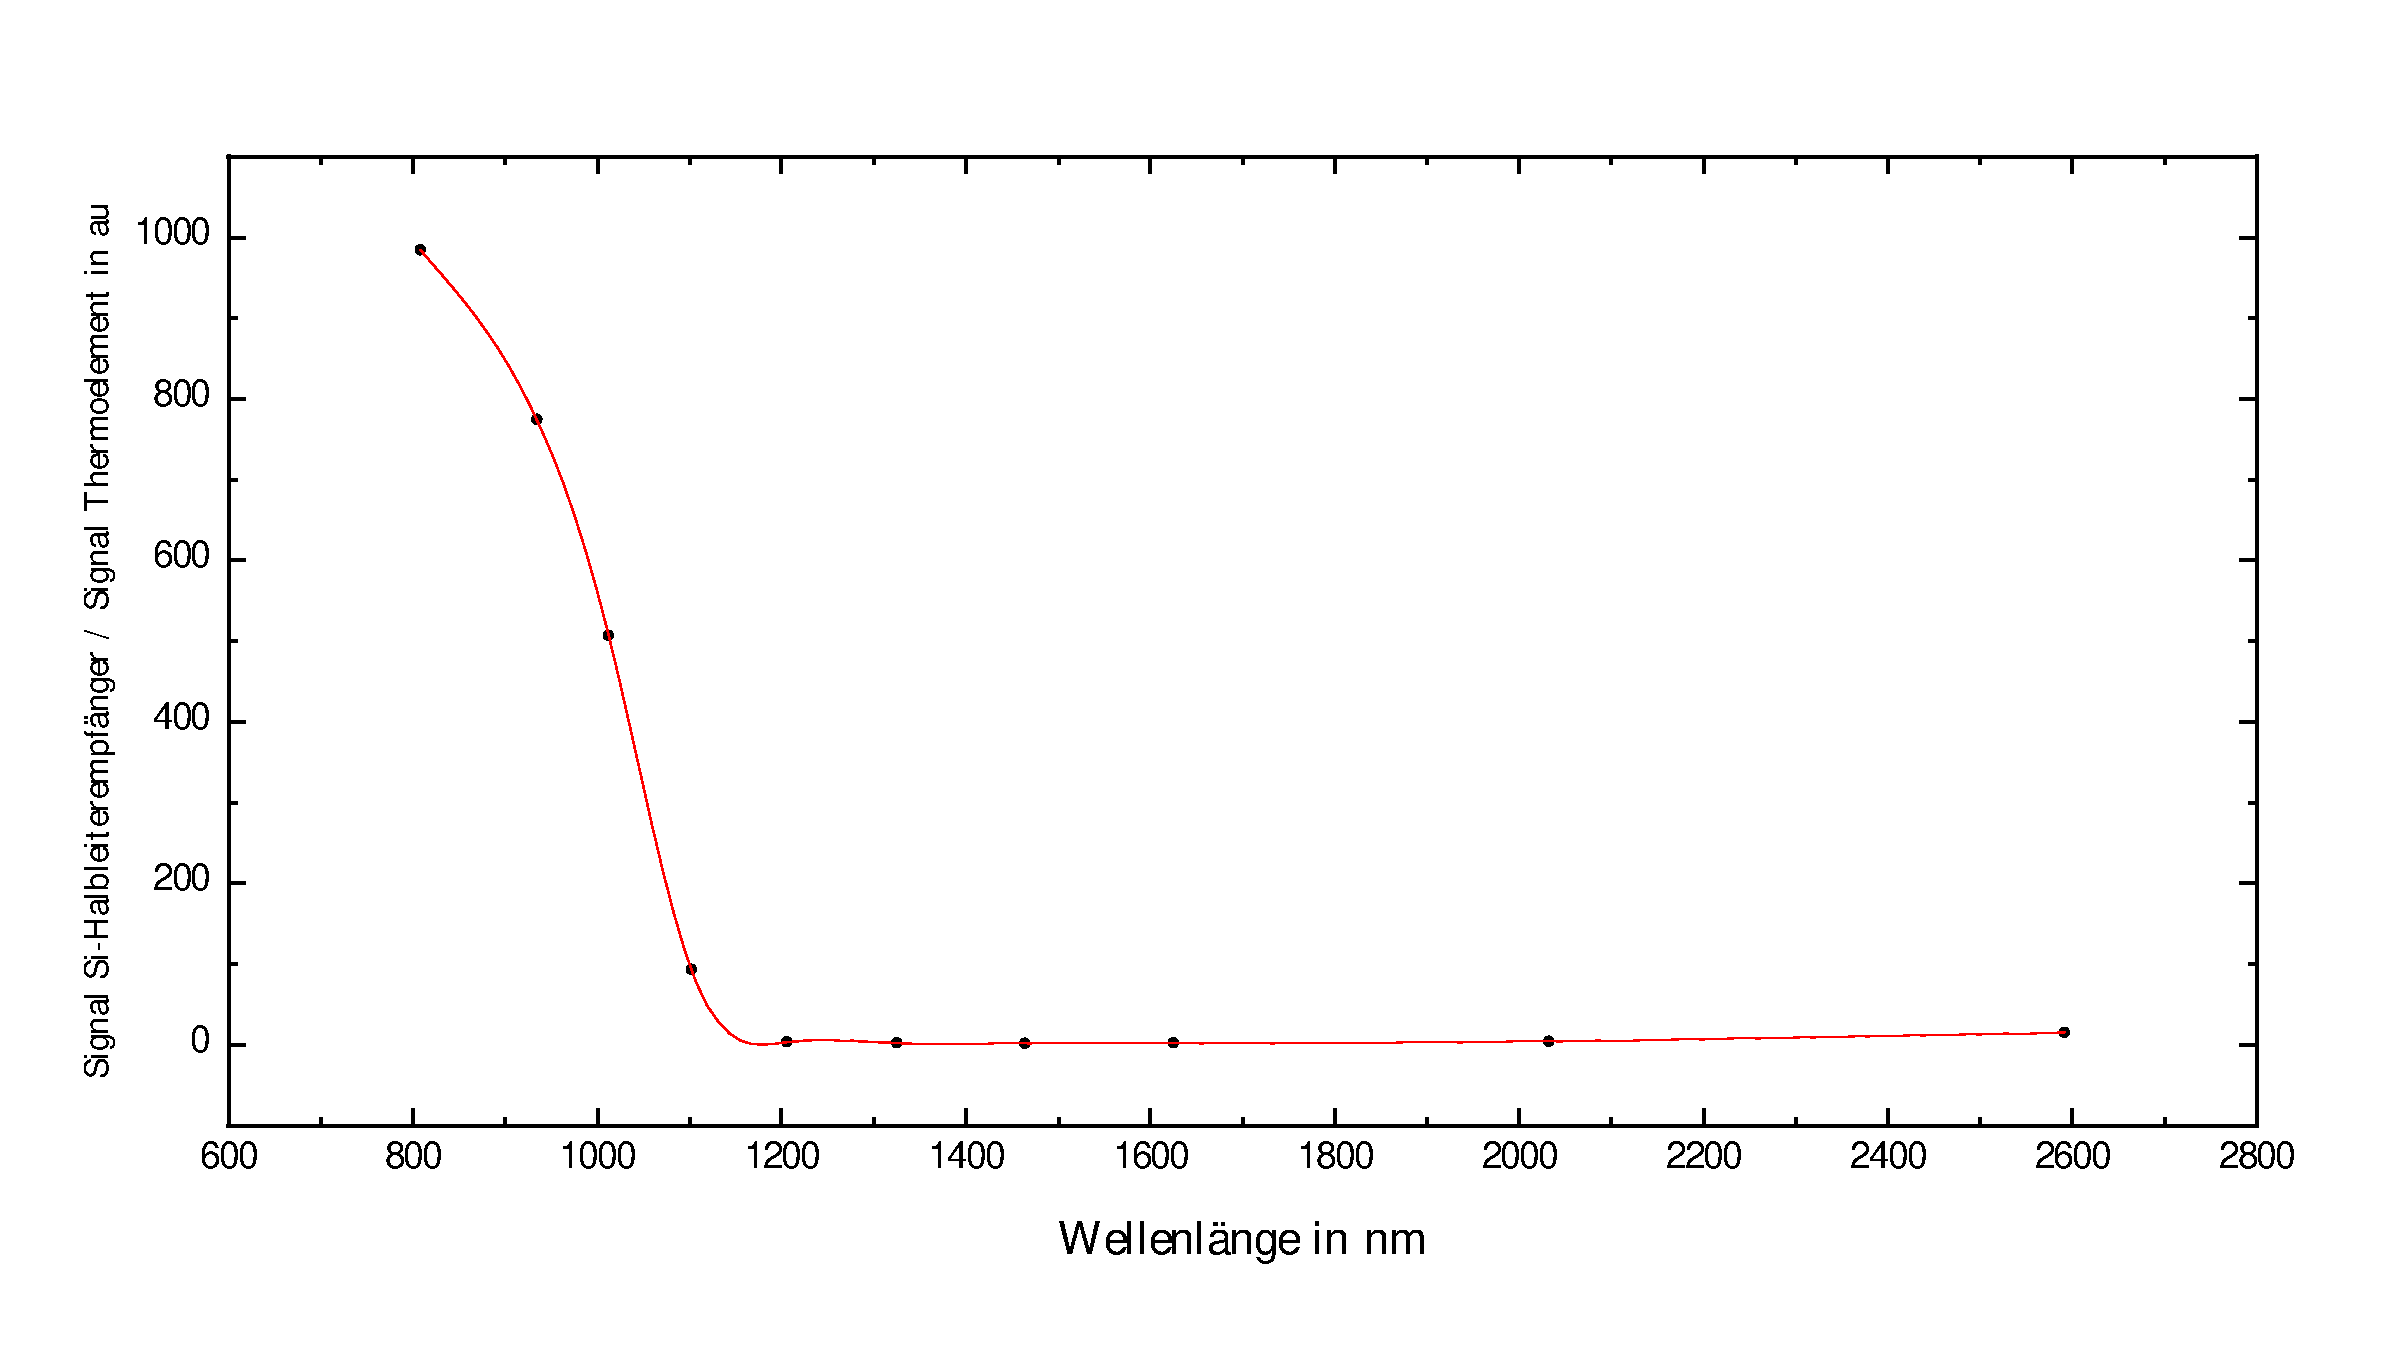
\includegraphics[width=\textwidth]{Bilder/Empfindlichkeit_SI.pdf}
    \caption{aus Messdaten}
  \end{subfigure}
  \begin{subfigure}{0.7\textwidth}
    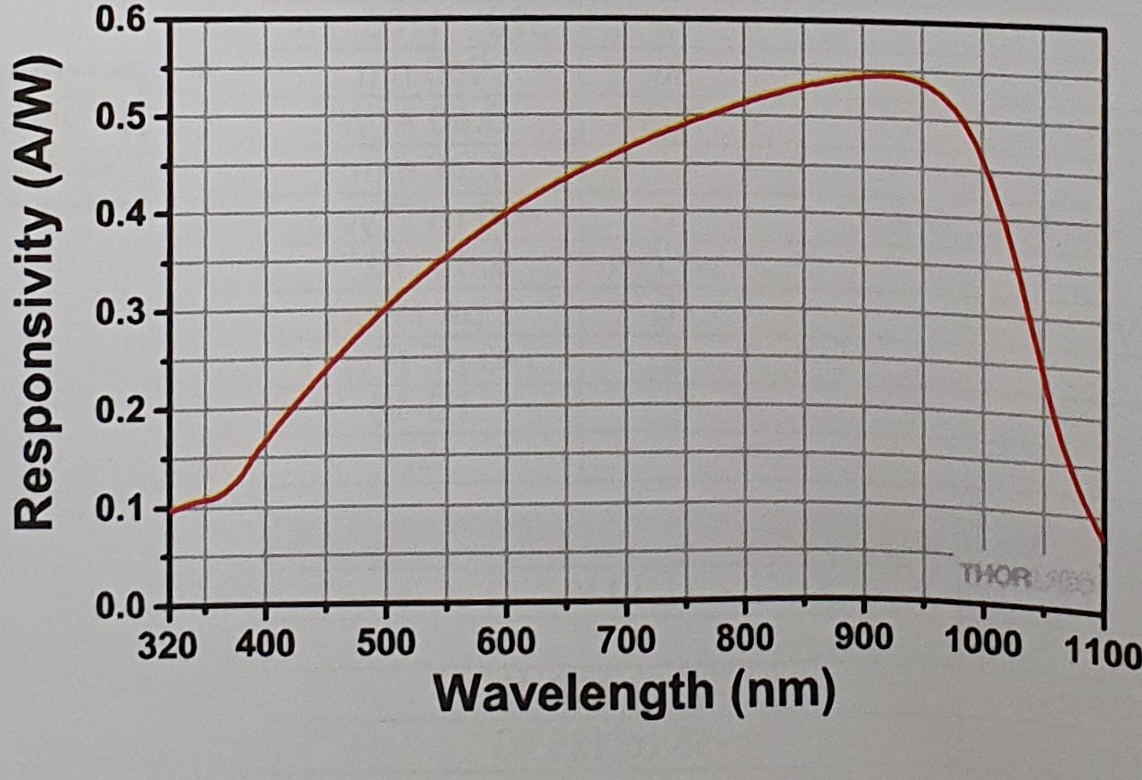
\includegraphics[width=\textwidth]{Bilder/Empfindlichkeit_SIHalbleiter_manual.jpeg}
    \caption{vom Hersteller}
  \end{subfigure}\hspace{1cm}
  \caption{spektrale Empfindlichkeit eines Si-Halbleiterdetektors}
  \label{fig:Empf_Si}
\end{figure}

\FloatBarrier

Es wird festgestellt, dass die Bereiche die aufgrund der Auflösung vermessbar sind, gut mit den vom Hersteller angegebenen Verlauf übereinstimmen. \\
Es zeigt sich deutlich, dass die Empfindlichkeit des Empfängers stark von der Wellenlänge abhängig ist, weshalb bei jeder Messung zu überlegen ist, in welchem Spektralbereich die zu vermessenden Werte liegen und daraus den passenden Halbleiterdetektor zu wählen ist. Wie in Abschnitt \ref{sec:Empfänger)} beschrieben, ergibt sich der Abknickpunkt als Bandlückenenergie des jeweiligen Halbleiters. Auch dies kann anhand der Messwerte des Siliziums bestätigt werden. Die Bandlückenenergie von Silizium bei \SI{300}{\kelvin} liegt bei \SI{1.12}{\electronvolt}. Dies entspricht einer Wellenlänge von \SI{1.11}{\micro\meter}. Der vermessene Abknickpunkt liegt in diesem Bereich.

\subsubsection{spektrale Energieverteilung einer Wolframlampe}
Für diese Messung wird das SPM2 verwendet.
\paragraph{Eichung SPM2}\label{par:EichungSPM2} Das SPM2 enthält eine eingebaute Wellenlängenanzeige. Diese wird verwendet, um auch die digitalisierten Daten zu eichen. Dazu wird in vorher festgelegten regelmäßigen Abständen bei der Aufnahme der Daten ein Marker gesetzt. Aus diesem Marker sowie der Kenntnis des Abstandes, in dem die Marker gesetzt werden, lassen sich Wellenlängen-Samplezahl Paare finden, womit eine Eichfunktion, also der Zusammenhang zwischen Sample und Wellenlänge, rekonstruiert werden kann und damit dann die Sampleanzahl in eine Wellenlänge umgerechnet wird.

Als Strahlungsquelle dient eine Wolframlampe, die bei einer Betriebsspannung von \SI{2}{V} und \SI{5}{V} betrieben wird. Die spektrale Energieverteilung wird mit einem Thermoelement, das an einen Lock-In-Verstärker angeschlossen ist, detektiert. Zu beachten ist hier die Theorie der spektralen Spaltbreite, die in \ref{sec:spektraleSpaltbreite} eingeführt wurde. Aufgrund der wellenlängenabhängigen Brechung des Prismas sind die mit der konstanten geometrischen Spaltbreite erfassten Wellenlängenbereiche unterschiedlich breit. Dies erfordert die Korrektur der gemessen Werte, indem durch $\Delta \lambda$ dividiert wird, um diese mit dem Planckspektrum vergleichen zu können. Für $\Delta \lambda$ gilt
\begin{align}
  \Delta \lambda = const* \frac{d\lambda}{dl}
\end{align}

wobei dl die Verschiebung der Mikrometerschraube ist.
$\frac{d\lambda}{dl}$ wird durch die Ableitung der oben beschriebenen Eichfunktion erhalten.\\

Aus den gemessenen Spektren wird mit Hilfe des \textsc{Wien}'schen Verschiebungsgesetzes die Temperatur der Wolframlampe berechnet. Hierzu wird das Maximum der gemessenen Verteilung bestimmt sowie die dazugehörige Wellenlänge. Über die Gleichung \ref{equ:WienscheVerschiebung} wird dann die Temperatur gewonnen. \\
Mit dieser Temperatur lässt sich die theoretische Planckkurve nach Gleichung \ref{eqn:2.1} berechnen.

\begin{figure}[htp]
  \centering
  \begin{subfigure}{0.9\textwidth}
    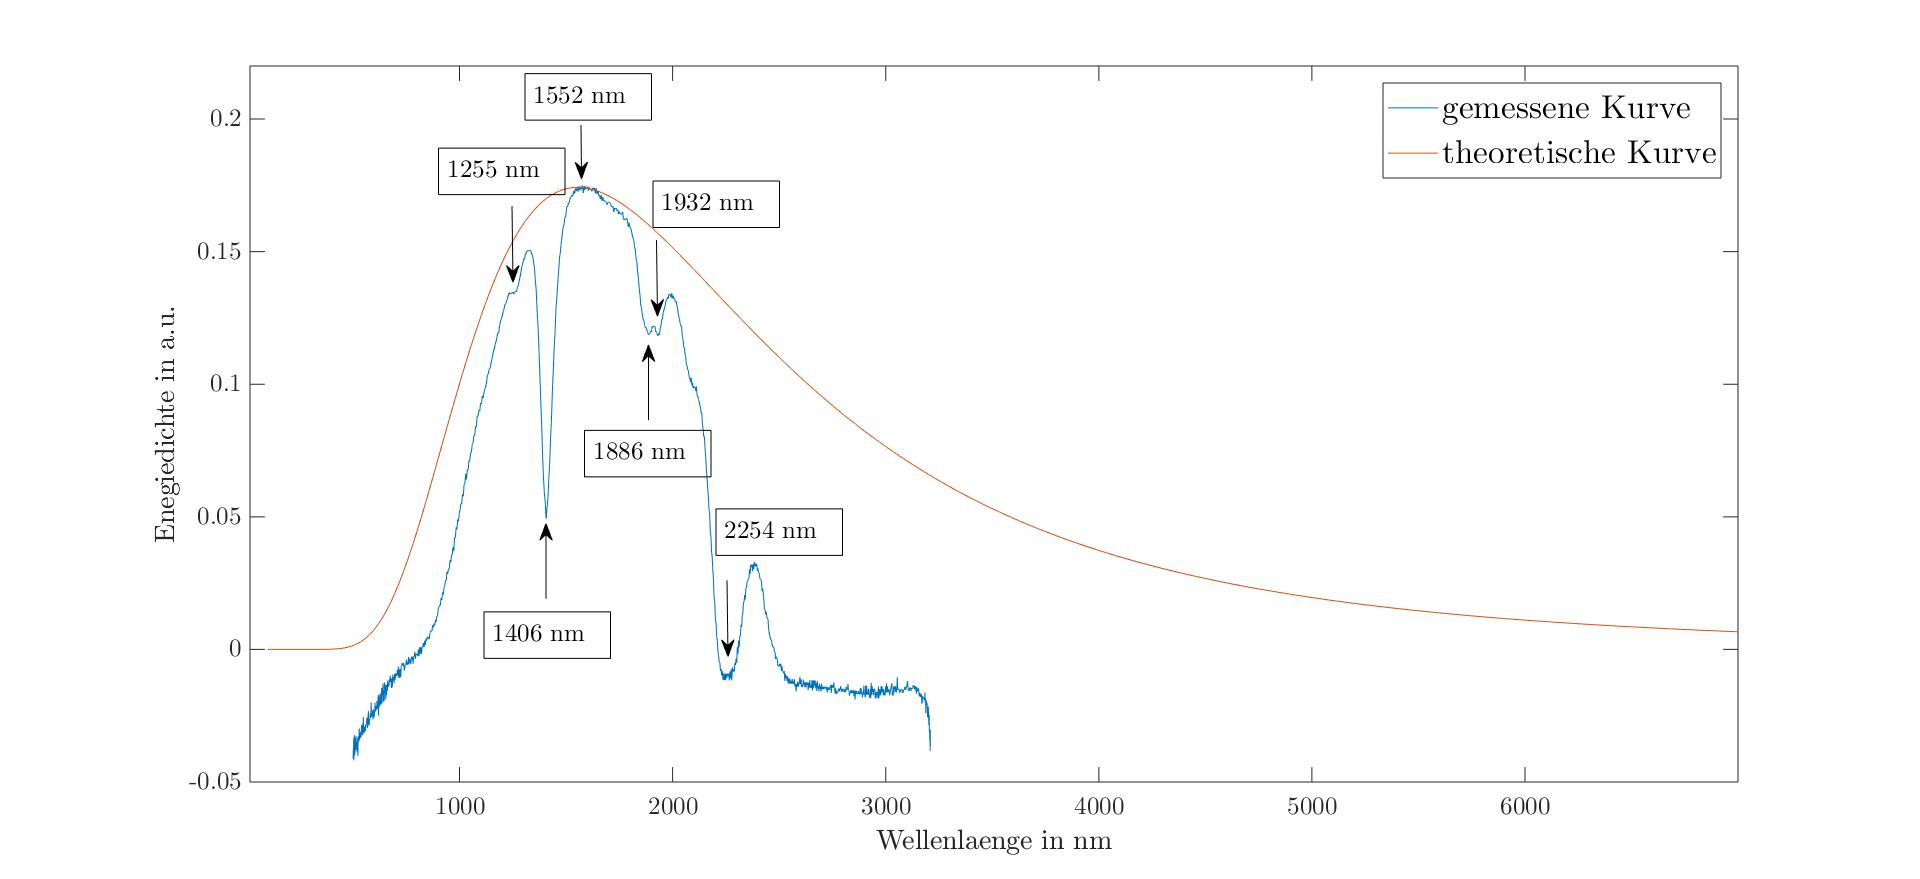
\includegraphics[width=\textwidth]{Bilder/Wolframlampe2V.jpg}
    \caption{Betriebsspannung = \SI{2}{\volt}}
  \end{subfigure}
  \begin{subfigure}{0.9\textwidth}
    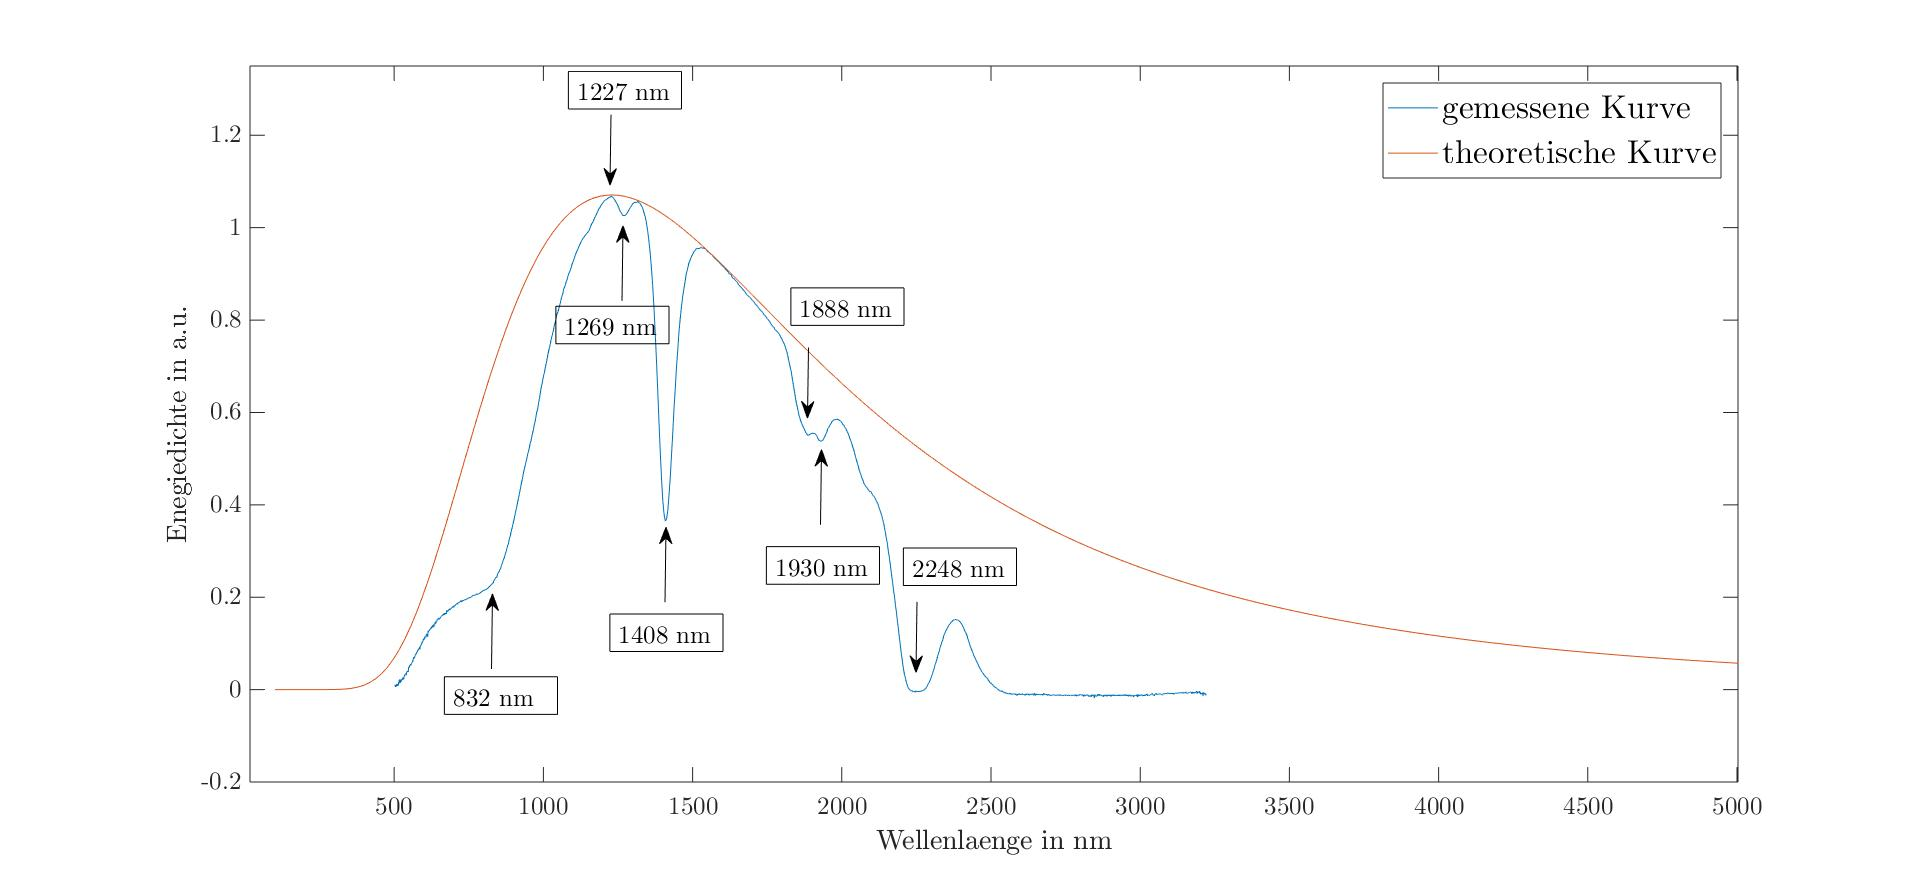
\includegraphics[width=\textwidth]{Bilder/Wolframlampe5V.jpg}
    \caption{Betriebsspannung = \SI{5}{\volt}}
  \end{subfigure}\hspace{0.5cm}
  \caption{spektrale Energiedichte einer Wolframdampflampe bei unterschiedlichen Betriebsspannungen}
  \label{fig:Wolframlampe}
\end{figure}

\FloatBarrier
An den Grafiken ist zu erkennen, dass die Messwerte dem in Abbildung \ref{fig:Planck} dargestellten Verhalten folgen. Für höhere Temperaturen schiebt sich das Maxima zu kleineren Wellenlängen, außerdem wird die Kurve höher. Die theoretische Kurve passt bei \SI{5}{\volt} Betriebsspannung sehr gut mit den gemessenen Werten überein. Bei \SI{2}{\volt} bestätigt sich der prinzipielle Verlauf, wenn auch die Kurve schmaler ist, als die Theoriekurve.\\
Der gemessene Galvanometerausschlag ergibt sich aus der Strahlungsdichte, einem Dispersionsanteil, sowie der Transmissionsfunktion. Durch Letztere wird berücksichtig, dass die sich im Strahlengang befindlichen Stoffe, wie z.B. die Aluminiumspiegel sowie das Prisma und die Luft, Strahlung absorbieren bzw. reflektieren können. An den Grafiken sind die Wellenlängen, bei denen es zu Absorption deutlich sichtbar. So finden sich in den Messungen die Absorptionsbanden von \ce{H2O} und \ce{CO2}, die theoretisch bei \SI{1.38}{\micro\meter} und \SI{1.87}{\micro\meter} liegen bei \SI{1.41}{\micro\meter} und \SI{1.89}{\micro\meter} für \SI{2}{\volt} bzw. \SI{5}{\volt}. Auch die Absorption der Aluminiumspiegel, die theoretisch bei \SI{0.85}{\micro\meter} liegt, tritt im Spektrum bei \SI{0.83}{\micro\meter} auf.
%DIE ANDEREN WERTE???

\subsection{Spektroskopische Messungen mit dem SPM2}

Die Aufnahme der Spektren mit dem SPM2 erfolgte über einen Lock-In-Verstärker und AD-Wandler digital. Dabei wurden drei verschiedene Prismen (Quarzglas \ce{SiO2}, \ce{NaCl} und \ce{KBr}) verwendet, die für verschiedene Bereiche des infraroten Spektrums transparent sind. Als breitbandige Strahlungsquellen stehen eine Wolframlampe und ein Keramikstrahler bereit. Das Spektrum des Keramikstrahlers befindet sich zum größten Teil im infraroten Spektrum und ist nicht sichtbar, was die Justage vor große Herausforderungen stellt.

Zunächst wurden zur Aufzeichnung der Referenz die Spektren der Wolframlampe mithilfe des Prismas aus Quarzglas und das Spektrum des Keramikstrahlers mithilfe der \ce{NaCl} und \ce{KBr} Prismen bei einer angelegten Spannung von \SI{19.4}{\volt} aufgenommen. Die Spektren sind in Abbildung~\ref{fig:Referenzspektren} dargestellt.

\begin{figure}[htp]
  \centering
  \begin{tikzpicture}
    \begin{axis}[width=0.98\textwidth, height=6cm, ylabel=Energiedichte in a.u., xlabel=Wellenlänge $\lambda$ in \si{\micro\metre},xmin=500, xmax=13000, legend cell align={left}, scaled x ticks={real:1000}, xtick scale label code/.code={}]
      \addplot[blue, thick] file[x index=1,y index=2]{Daten/Kalibrierung_Wolframlampe500-3200nm.txt};
      \addlegendentry{Wolframlampe \ce{SiO2}}
      \addplot[orange, thick] file[x index=1,y index=2]{Daten/Kalibrierung_NaClPrisma_Keramikstrahler_19_4V_3_6Grad_600nm_bis11_5mu_all200nmMaker_Spalt_1500mu_gut.txt};
      \addlegendentry{Keramikstrahler NaCl}
      \addplot[green!50!black, thick] file[x index=1,y index=2]{Daten/Kalibrierung_KBrPrisma_Keramik19_4V_3_6Grad_1500nm_all500nmMaker_Spalt_1500mu.txt};
      \addlegendentry{Keramikstrahler KBr}
    \end{axis}
  \end{tikzpicture}
  \caption{Referenzspektren der Wolframlampe (blau) und des Keramikstrahlers (orange, grün) unter Verwendung verschiedener Prismen. Das Maximum der Strahlungsleistung liegt für den Keramikstrahler bei höheren Wellenlängen.}
  \label{fig:Referenzspektren}
\end{figure}


\subsubsection{Molekülschwingungsbanden von Ethanoldampf}
Zur Untersuchung der Schwingungsbanden von Ethanoldampf wurde ein Glasrohr in der Mitte mit Ethanol gefüllt und mithilfe des Keramikstrahlers ein Transmissionsspektrum aufgenommen, welches anschließend mit einem Referenzspektrum verglichen wurde. Beide Spektren sind im Vergleich in Abbildung~\ref{fig:Ethanoldampf} dargestellt.

\begin{figure}[htp]
  \centering
  \begin{tikzpicture}
    \begin{axis}[disabledatascaling, width=\textwidth, height=6cm, ylabel=Spannung U in \si{\volt}, xlabel=Wellenlänge $\lambda$ in \si{\micro\metre}, xmin = 600, xmax=12400, scaled x ticks={real:1000}, xtick scale label code/.code={}, legend cell align={left}]
      \addplot[blue, thick] file[x index=1,y index=2]{Daten/Kalibrierung_NaClPrisma_Keramikstrahler_19_4V_3_6Grad_600nm_bis11_5mu_all200nmMaker_Spalt_1500mu_gut.txt};
      \addlegendentry{Transmissionsspektrum ohne Ethanol}
      \addplot[orange, thick] file[x index=1,y index=2]{Daten/Kalibrierung_NaClPrisma_Keramikstrahler_19_4V_Ethanoldampf_3_6Grad_600nm_bis11_5mu_all200nmMaker_Spalt_1500mu.txt};
      \addlegendentry{Transmissionsspektrum mit Ethanol}
    \end{axis}
  \end{tikzpicture}
  \caption{Aufgenommenes Transmissionsspektrum von Ethanoldampf mit einem NaCl Spektrometer und einer Spaltbreite von \SI{1.5}{\milli\metre}.}
  \label{fig:Ethanoldampf}
\end{figure}


Die Spektren wurden jeweils geglättet, um den Einfluss des Rauschens des Lock-In-Verstärkers zu reduzieren. Die Absorptionsrate des Ethanoldampfes ist in Abbildung~\ref{fig:Absorption_Ethanol} dargestellt. Dort ist in grau die Absorptionsrate für die ungeglätteten Kurven der Transmissionsspektren abgebildet. Es zeigt sich, dass die Glättung den qualitativen Verlauf nicht ändert.

\begin{figure}[htp]
  \centering
  \begin{tikzpicture}
    \begin{axis}[disabledatascaling, width=\textwidth, height=6cm, ylabel=Absorptionsrate, xlabel=Wellenlänge $\lambda$ in \si{\micro\metre}, xmin = 1100, xmax=10200, ymin = 0, ymax = 1.1, scaled x ticks={real:1000}, xtick scale label code/.code={}]
      \addplot[black!50!white, thick, opacity=0.5] file[x index=1,y index=2]{Daten/Kalibrierung_Absorption_NaClPrisma_Keramikstrahler_19_4V_Ethanoldampf_3_6Grad_600nm_bis11_5mu_all200nmMaker_Spalt_1500mu.txt};
      \addplot[blue, thick] file[x index=1,y index=2]{Daten/Absorption_Smooth_Kalibrierung_NaClPrisma_Keramikstrahler_19_4V_Ethanoldampf_3_6Grad_600nm_bis11_5mu_all200nmMaker_Spalt_1500mu.txt};
      \draw[<-,thick](3517,0.690) -- +(0,-0.15)node[left, rotate=90]{\footnotesize 3,459};
      \draw[<-,thick](7200,0.514) -- +(0,-0.15)node[left, rotate=90]{\footnotesize 7,200};
      \draw[<-,thick](8027,0.527) -- +(0,-0.15)node[left, rotate=90]{\footnotesize 8,027};
      \draw[<-,thick](9422,0) -- +(0,0.15)node[right, rotate=90]{\footnotesize 9,422};
    \end{axis}
  \end{tikzpicture}
  \caption{Aufgenommenes Absorptionsspektrum von Ethanoldampf mit einem NaCl Spektrometer und einer Spaltbreite von \SI{1.5}{\milli\metre}.}
  \label{fig:Absorption_Ethanol}
\end{figure}


\begin{wrapfigure}{r}{4.5cm}
  \centering
  \chemfig{C(-[:90]H)(-[:180]H)(-[:270]H)-C(-[:90]H)(-[:270]H)-OH}
  \caption{Ethanol}
\end{wrapfigure}
Im Bereich von \SIrange{2}{10}{\micro\metre} wurden insgesamt vier Absorptionsbanden registriert, die auf Molekülschwingungen zurückzuführen sind. Bei Ethanol handelt es sich um einen Alkohol mit der nebenstehend abgebildeten Strukturformel und der Summenformel \ce{C2H5OH}. Bei dem ersten Peak handelt es sich wahrscheinlich um eine Valenzschwingung einer \ce{OH}- oder \ce{CH} Gruppe~\cite{Roempp}. Beide Schwingungsarten treten im beobachteten Wellenlängenbereich auf. Bei dem zweiten Peak bei \SI{7.2}{\micro\metre} wurden als mögliche Schwingungsbanden Deformationsschwingungen der \ce{CC}- oder \ce{CH} Gruppen zugeordnet~\cite{Roempp}. Die letzten beiden Peaks wurden einer \ce{COH}-Deformationsschwingung und einer \ce{CO}-Streckschwingung zugeordnet~\cite{Gunzler}. Die jeweiligen Wellenlängenbereiche sind in Tabelle~\ref{tab:Ethanoldampf} aufgelistet.

\begin{table}[htp]
  \centering
  \caption{Wellenlängenbereiche der zugeordneten Molekülschwingungen.}
  \begin{tabular}{c c c c}
    \toprule
    $\lambda_\text{gemessen}$ in \si{\micro\metre} & $\lambda_\text{Literatur}$ in \si{\micro\metre} & $\nu_\text{Literatur}$ in \si{\per\centi\metre} & Schwingungsart \\
    \midrule
    3,459 & 3,2-4,2 & 2400-3200 & \ce{OH}-Streckschwingung \\
          & 3,4-3,5 & 2850-2960 & \ce{CH}-Streckschwingung \\
    7,200 & 7,2-7,3 & 1370-1385 & \ce{CC}-Deformationsschwingung \\
          & 6,8-7,4 & 1350-1470 & \ce{CH}-Deformationsschwingung \\
    8,027 & 8,0-10,0 & 1000-1250 & \ce{COH}-Deformationsschwingung \\
    9,420 & 9,3-10,0 & 1000-1075 & \ce{CO}-Streckschwingung
  \end{tabular}
  \label{tab:Ethanoldampf}
\end{table}

Es muss jedoch noch angemerkt werden, dass bei der Messung Fehler auftreten können, da im verwendeten Rohr, in dem sich der Ethanoldampf befand, ebenfalls Absorption an den Glas auftreten kann. Von daher wäre es ratsam gewesen, eine weitere Referenzmessung mit dem Rohr im Strahlengang durchzuführen.
\FloatBarrier

\subsubsection{Absorptionsspektren von Kunststoffen}

Zwei weitere, mit dem SPM2 vermessene Proben bestanden aus im sichtbaren Spektralbereich durchsichtigen Kunsstoffen. Dabei handelt es sich einerseits um eine durchsichtige Folie aus Polypropylen, welche mit der Folie der Praktikumsanleitung vergleichbar ist und andererseits um eine Acetatfolie. Die Folien wurden in den Strahlengang gestellt und die auftretende Absorption gemessen.

\begin{figure}[htp]
  \centering
  \begin{tikzpicture}
    \begin{axis}[width=0.98\textwidth, height=6cm, ylabel=Spannung U in \si{volt}, xlabel=Wellenlänge $\lambda$ in \si{\micro\metre}, xmin = 1000, xmax=13000, xtick={}, legend cell align={left}, scaled x ticks={real:1000}, xtick scale label code/.code={}]
      \addplot[blue, thick] file[x index=1,y index=2]{Daten/Kalibrierung_KBrPrisma_Keramik19_4V_Si02_Reflexionsmessung_Referenzmessung_Silberspiegel_1_8Grad_1500nm_all500nmMaker_Spalt_1500mu.txt};
      \addlegendentry{Referenzmessung}
      \addplot[orange, thick] file[x index=1,y index=2]{Daten/Kalibrierung_KBrPrisma_Keramik19_4V_Polypropylen_3_6_Grad_1000nm_all500nmMaker_Spalt_1500mu_inReflexionsstellunggemessen.txt};
      \addlegendentry{Polypropylen}
      \addplot[green!50!black, thick] file[x index=1,y index=2]{Daten/Kalibrierung_KBrPrisma_Keramik19_4V_Acetat_3_6_Grad_1000nm_all500nmMaker_Spalt_1500mu_inReflexionsstellunggemessen.txt};
      \addlegendentry{Acetatfolie}
    \end{axis}
  \end{tikzpicture}
  \caption{Transmissionsspektrum verschiedener Kunststoffe. In blau ist die Referenzmessung ohne Probe dargestellt.}
  \label{fig:Kunststoffe}
\end{figure}


Die Transmissionsrate ergibt sich wieder als der Quotient aus gemessenem Spektrum gegenüber der Referenzkurve und ist in Abbildung~\ref{fig:Absorption_Kunststoffe} dargestellt. Wird die Transmissionsrate mit den für Ethanoldampf aufgenommen Spektren verglichen, so ergeben sich hier Molekülschwingungen in den gleichen Bereichen, nämlich Streckschwingungen von \ce{OH}- und \ce{CH}-Gruppen im Bereich von \SIrange{3}{4}{\micro\metre} und für das Polypropylen Deformationsschwingungen bei \SI{7.2}{\micro\metre}.

\begin{figure}[htp]
  \centering
  \begin{tikzpicture}
    \begin{axis}[ width=0.98\textwidth, height=6cm, ylabel=Transmissionsrate, xlabel=Wellenlänge $\lambda$ in \si{\micro\metre}, xmin = 1500, xmax=13000, ymin = 0, ymax = 1.1, scaled x ticks={real:1000}, xtick scale label code/.code={}, legend cell align={left}]
      \addplot[black!50!white, thick, opacity=0.5] file[x index=1,y index=2]{Daten/Absorption_Kalibrierung_KBrPrisma_Keramik19_4V_Polypropylen_3_6_Grad_1000nm_all500nmMaker_Spalt_1500mu_inReflexionsstellunggemessen.txt};
      \addlegendentry{}
      \addplot[black!50!white, thick, opacity=0.5] file[x index=1,y index=2]{Daten/Absorption_Kalibrierung_KBrPrisma_Keramik19_4V_Acetat_3_6_Grad_1000nm_all500nmMaker_Spalt_1500mu_inReflexionsstellunggemessen.txt};
      \addplot[orange, thick] file[x index=1,y index=2]{Daten/Absorption_Smooth_Kalibrierung_KBrPrisma_Keramik19_4V_Polypropylen_3_6_Grad_1000nm_all500nmMaker_Spalt_1500mu_inReflexionsstellunggemessen.txt};
      \addlegendentry{}
      \addplot[green!50!black, thick] file[x index=1,y index=2]{Daten/Absorption_Smooth_Kalibrierung_KBrPrisma_Keramik19_4V_Acetat_3_6_Grad_1000nm_all500nmMaker_Spalt_1500mu_inReflexionsstellunggemessen.txt};
      \legend{, ,Polypropylen, Acetat};
    \end{axis}
  \end{tikzpicture}
  \caption{Aufgenommene Transmissionsrate verschiedener Kunststoffe. In grau ist jeweils die Kurve für das ungeglättete Lock-In-Signal dargestellt.}
  \label{fig:Absorption_Kunststoffe}
\end{figure}


\FloatBarrier
\subsubsection{Bestimmung der Bandlückenenergie von Halbleitern}

Im Folgenden werden die Transmissionsspektren von zwei zunächst unbekannten Halbleitern untersucht. Zur Verfügung standen hierfür zwei kreisförmige, im sichtbaren Spektrum undurchsichtige, Halbleiterproben. Die Plättchen wurden zur Transmissionsmessung in den Strahlengang gestellt. Die Messergebnisse sind qualitativ in Abbildung~\ref{fig:Halbleitermessung} dargestellt.

\begin{figure}[htp]
  \centering
  \begin{tikzpicture}
    \begin{axis}[disabledatascaling, width=\textwidth, height=6cm, ylabel=Spannung U in \si{volt}, xlabel=Wellenlänge $\lambda$ in \si{\nano\metre}, xmin = 500, xmax=3250, xtick={}, legend cell align={left}]
      \addplot[blue, thick] file[x index=1,y index=2]{Daten/Kalibrierung_Wolframlampe500-1200nm.txt};
      \addlegendentry{Referenzmessung}
      \addplot[orange, thick] file[x index=1,y index=2]{Daten/Kalibrierung_Glasprisma_Wolframlampe5V_kleinesHalbleiterplaettchen_3_6Grad_500nm_all100nmMaker_Spalt_500mu.txt};
      \addlegendentry{Silizium}
      \addplot[green!50!black, thick] file[x index=1,y index=2]{Daten/Kalibrierung_Glasprisma_Wolframlampe5V_mitgrossemHalbleiterplaettchen_3_6Grad_500-3200nm_mitMarkern2_Spalt_500mu.txt};
      \addlegendentry{Galiumarsenid}
    \end{axis}
  \end{tikzpicture}
  \caption{Transmissionsspektren von Silizium und Galiumarsenid im Vergleich zu einer Referenzmessung. Es muss jedoch beachtet werden, dass zur Aufnahme der Transmissionsspektren von Si und GaAs eine höhere Verstärkung im Lock-In verwendet wurde, was einen quantitativen Vergleich der Kurven erschwert.}
  \label{fig:Halbleitermessung}
\end{figure}


Zur besseren Diskussion der Spektren wurden diese durch das in blau dargestellte Spektrum der Referenz geteilt. Dadurch ergibt sich die Absorptionsrate der Halbleiter als relative Größe. Zur Bestimmung der Bandlückenenergie wird der Punkt gesucht, ab der die Transmissionsrate ansteigt, denn erst Photonen mit einer Energie, die kleiner als die Bandlücke ist, werden von der Probe mit einer Dicke von \SIrange{1}{2}{\milli\metre} nicht mehr absorbiert und können detektiert werden Die entsprechende Grenzwellenlänge ist in Abbildung~\ref{fig:Halbleitermessung_relativ} mit eingezeichnet.

\begin{figure}[htp]
  \centering
  \begin{tikzpicture}
    \begin{axis}[disabledatascaling, width=\textwidth, height=6cm, ylabel=Absorptionsrate, xlabel=Wellenlänge $\lambda$ in \si{\nano\metre}, xmin = 950, xmax=2150, xtick={}, ymin =-.1, ymax = 1.15, legend cell align={left}]
      \filldraw[draw=white!80!orange,fill=white!90!orange] (1020,-.1) rectangle (1080,1.2);
      \draw[thick, white!50!orange] (1050,-.1) -- (1050,1.2);
      \filldraw[draw=green!50!black, draw opacity = 0.2,fill=green!50!black, fill opacity = 0.1] (1770,-.1) rectangle (1830,1.2);
      \draw[thick, green!50!black, opacity = 0.5] (1800,-.1) -- (1800,1.2);
      \addplot[orange, thick] file[x index=1,y index=2]{Daten/Absorption_Smooth_Kalibrierung_Glasprisma_Wolframlampe5V_kleinesHalbleiterplaettchen_3_6Grad_500nm_all100nmMaker_Spalt_500mu.txt};
      \addlegendentry{Silizium}
      \addplot[green!50!black, thick] file[x index=1,y index=2]{Daten/Absorption_Smooth_Kalibrierung_Glasprisma_Wolframlampe5V_mitgrossemHalbleiterplaettchen_3_6Grad_500-3200nm_mitMarkern2_Spalt_500mu.txt};
      \addlegendentry{Germanium}
    \end{axis}
  \end{tikzpicture}
  \caption{Transmissionsrate von Silizium und Germanium.}
  \label{fig:Halbleitermessung_relativ}
\end{figure}


Die beiden Grenzwellenlängen für den Beginn der Absorption lassen sich über die nach Einstein gegebene Beziehung $E = h \nu = \frac{h c}{\lambda}$ in eine Energie umrechnen. Danach ergibt sich
\begin{align}
  E_g(\ce{Si}) &= \frac{h c}{\SI{1050\pm50}{\nano\metre}} = \SI{1.181\pm0.056}{\electronvolt}\\
  E_g(\ce{Ge}) &= \frac{h c}{\SI{1800\pm50}{\nano\metre}} = \SI{0.689\pm0.019}{\electronvolt}.
\end{align}
Die in~\cite{Hunklinger} gegeben Literaturwerte für Silizium $E_g = \SI{1.12}{\electronvolt}$ und Germanium $E_g = \SI{0.66}{\electronvolt}$ bei einer Temperatur von \SI{300}{\kelvin} liegen innerhalb des angegebenen Fehlerintervalls.

\subsubsection{Absorption und Reflektivität von \ce{SiO2}}
\paragraph{Absorption}
Um die Absorption von \ce{SiO2} zu messen, wurde sowohl ein Plättchen aus undotiertem als auch ein Plättchen mit dotiertem \ce{SiO2} in den Strahlengang positioniert.
\begin{figure}[htp]
  \centering
    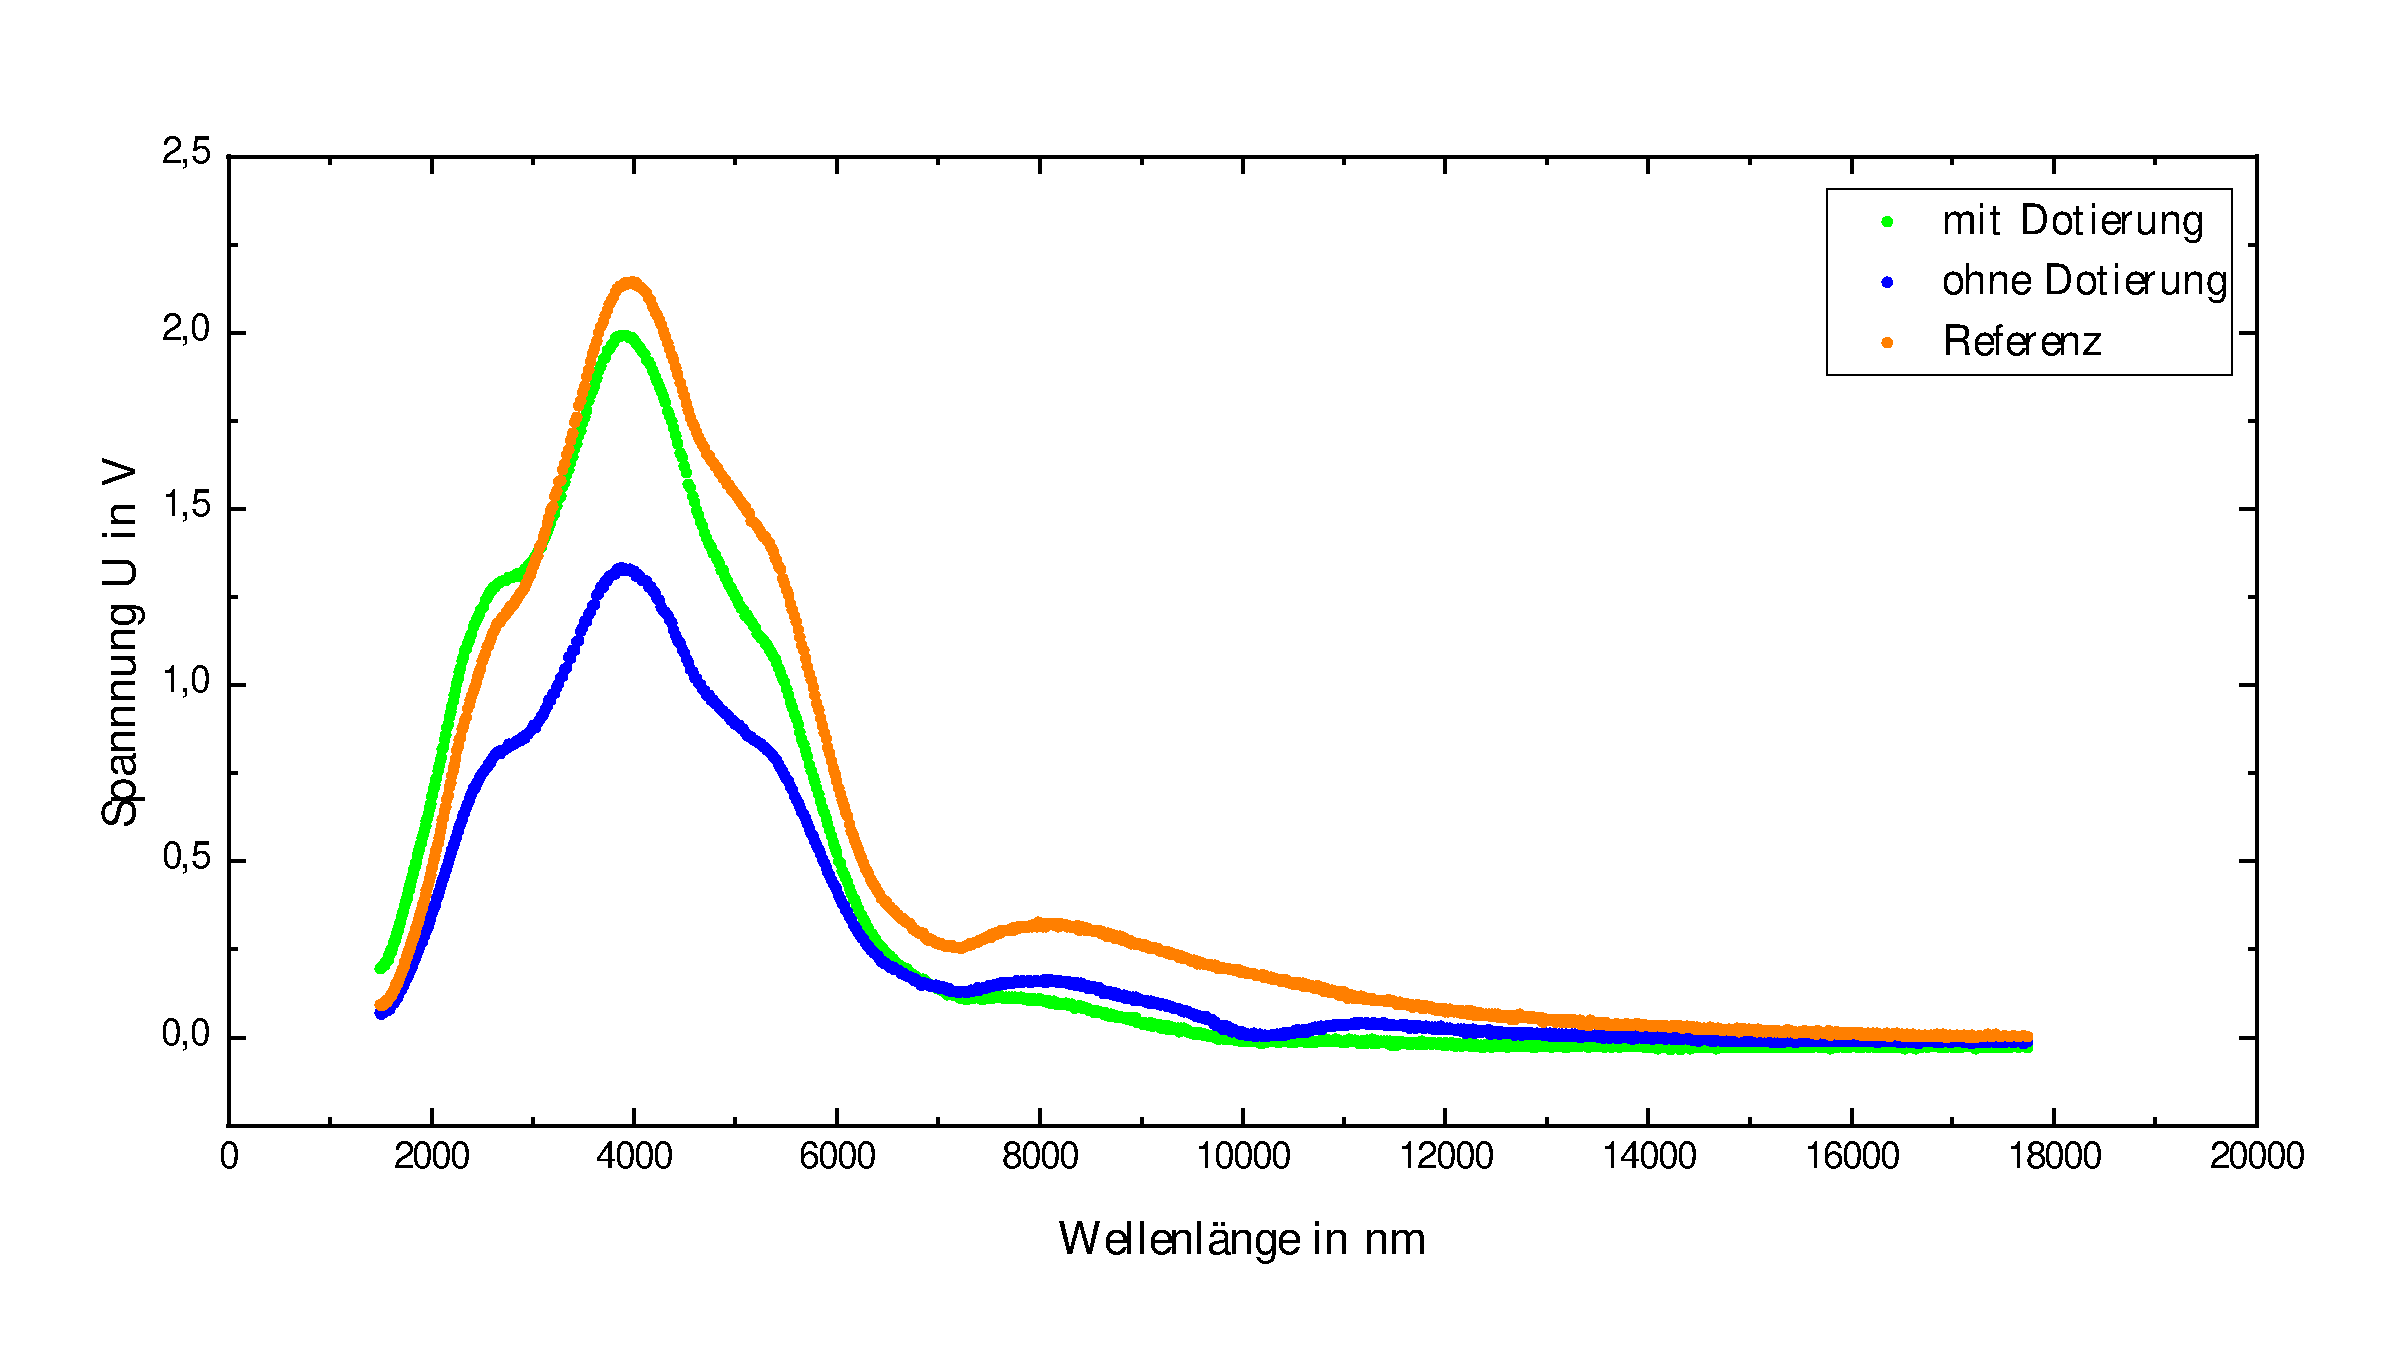
\includegraphics[width=\textwidth]{Bilder/AbsorptionSiO2.pdf}
    \caption{Signale am Thermoelement bei Plättchen mit dotiertem sowie mit undotierten \ce{SiO2} im Strahlengang sowie ohne Plättchen im Strahlengang}
\end{figure}
Um Gebiete mit Absorption besser kenntlich zu machen, wird das Verhältnis aus jeweiligem Signal zu Referenzsignal dargestellt.

\begin{figure}[htp]
  \centering
    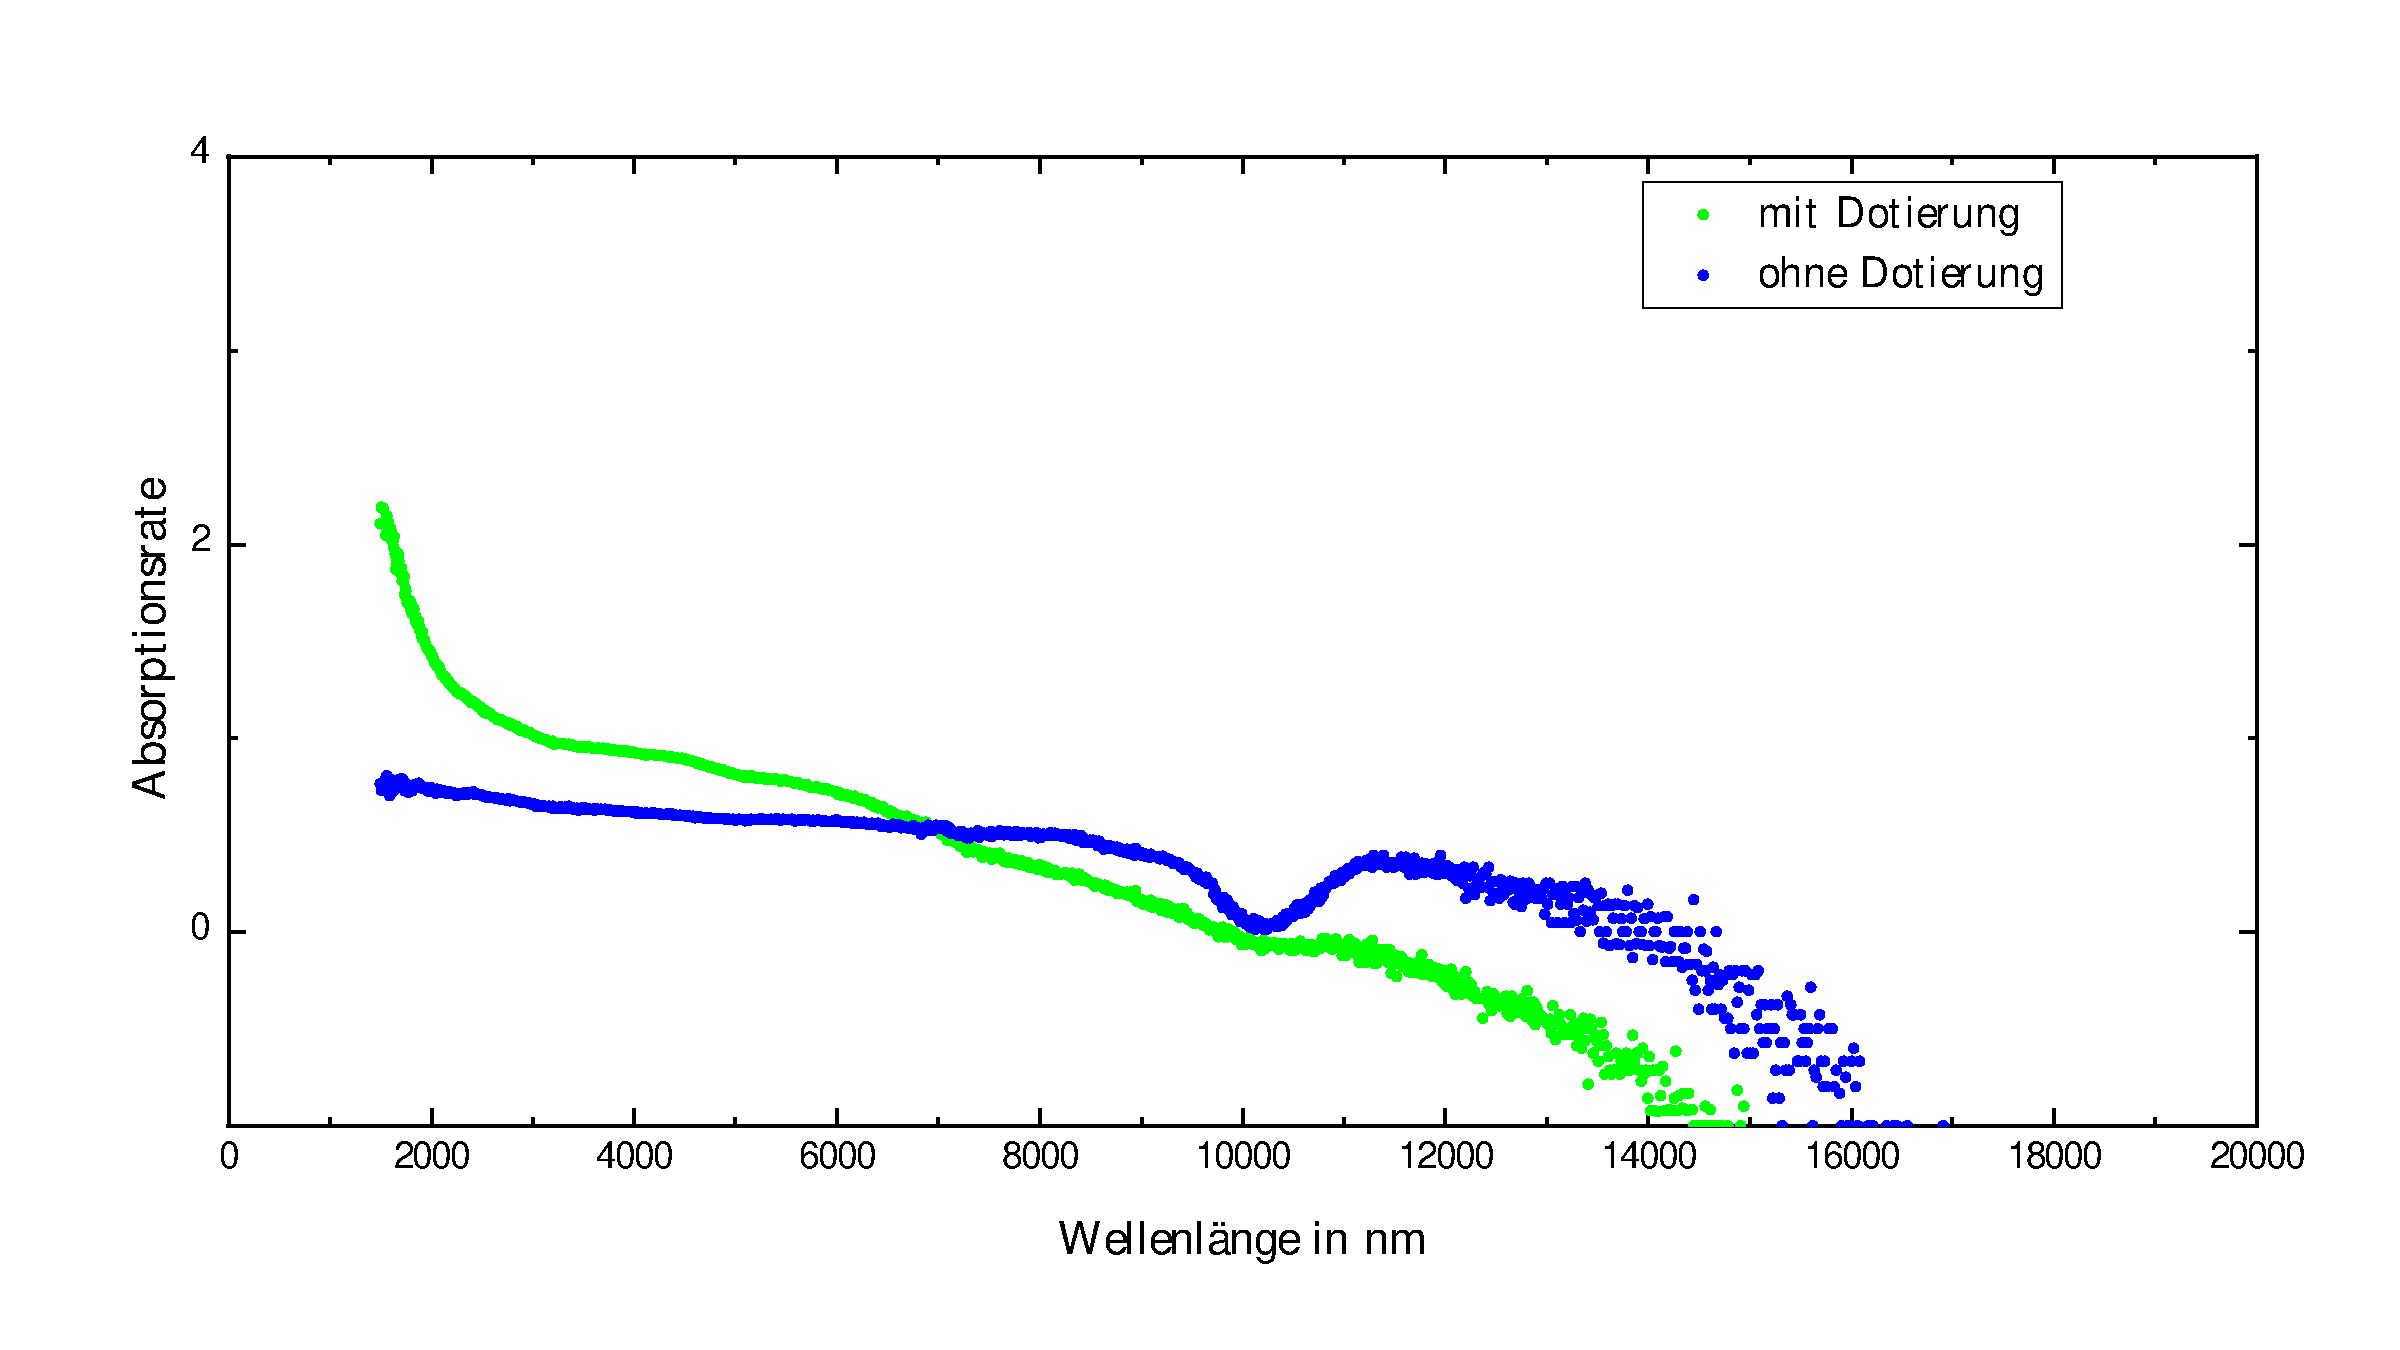
\includegraphics[width=\textwidth]{Bilder/Absorptionsrate_Si02.pdf}
    \caption{Verhältnis jeweiliges Signal zu Referenzsignal}
\end{figure}
\FloatBarrier
Der Bereich der Absorption ist beim undotierten Präparat im Strahlengang deutlich zu erkennen und liegt bei \SI{10.24}{\micro\meter}.

\paragraph{Reflexionsvermögen}
Für die Messung des Reflexionsvermögens wird der Aufbau teilweise geändert. Vom zweitem Spiegel wird der Strahl auf eine reflektierende Einheit gelenkt. Der Detektor ist so positioniert, um den reflektierten Anteil zu erfassen. Die Messung wird zweimal durchgeführt. Einmal mit einem komplett reflektierenden Aluminiumspiegel als reflektierendes Element (Referenz) und einmal ist an der exakt selben Stelle ein \ce{SiO2} Plättchen positioniert.
\begin{figure}[htp]
  \centering
    \includegraphics[width=\textwidth]{Bilder/Reflektivität_SiO2.pdf}
    \caption{Messungen des Signals nach Reflexion an \ce{SiO2} Plättchen bzw. an Aluminiumspiegel. Die Darstellung ist nicht maßstabsgetreuen. Zusätzlich ist die Reflexionsrate, also das Verhältnis aus Signal zu Referenz, dargestellt. Der zweite Peak des \ce{SiO2} Signal entspricht ungefähr \SI{50}{\percent} des ursprünglichen Signals. }
\end{figure}
\FloatBarrier
Wie an der Reflexionsrate zu erkennen ist, ist die Reflexion vor allem im Bereich um $\lambda = \SI{9.01}{\micro\meter}$ besonders groß. Obwohl hier der Referenzwert der reflektierten Strahlung sehr gering ist, wird fast genauso viel reflektiert, wie in dem Bereich, in dem die Referenz ihr deutliches Maximum trägt.\\

Wie in Abschnitt \ref{sec:AbsorptionundReflexion} diskutiert, sind die Wellenlängenbereiche hoher Absorption zugleich diese, in denen gut reflektiert wird. Das können die Messdaten teilweise bestätigen. Der Absorptionsbereich liegt im Bereich um \SI{10.24}{\micro\meter}, während der Reflexionsbereich um die \SI{9.01}{\micro\meter} lokalisiert ist. Die Größenordnung ist somit bei beiden Messungen die gleiche und es treten Überschneidungen der Bereiche auf. Die Abweichung lässt sich durch möglicherweise auftretenden Verunreinigungen des \ce{SiO2} auf den beiden unterschiedlichen Elementen sowie durch etwaige abweichende chemische Zusammensetzung oder Reinheit erklären.



% *********************************************
% ***** KAPITEL 5 *****************************
% *********************************************
\newpage
\section{Zusammenfassung}


% ***** Literaturverzeichnis ******************

\bibliography{Literatur}{}
\bibliographystyle{plain}
\end{document}
